\documentclass[10pt]{article}

\usepackage[top=1in, bottom=1in, left=1in, right=1in]{geometry}
\usepackage{graphicx}
\usepackage{tocbibind}
\usepackage{float}
\usepackage{fancyhdr}
\usepackage{bm}
\usepackage{amsmath,amssymb}
\usepackage{subfig}
\usepackage{booktabs}
\newcommand{\fig}{Fig.~\ref}
\newcommand{\figs}{Figs.~\ref}
\newcommand{\tab}{table~\ref}
\setlength{\parindent}{0mm}
\setlength{\parskip}{3mm}
\usepackage[numbers,square,sort&compress]{natbib}
\bibliographystyle{is-unsrt}

\title{\bf Bistable Curve Fitting}
\date{\vspace{-15ex}}

\begin{document}
\maketitle
\hrulefill

\section{Experimental fit}
The energy-displacement curves for the bistable elements can be fitted well with an eighth order polynomial. Therefore, each of these curves can be represented as a 2D slice of the following normalized 3D plot (with the origin shifted to one of the wells)
\begin{equation}
	\psi(u,d) = \sum_{n=2}^{8} C_{n}(d) \,\left(\tfrac{u}{\text{eq}(d)}\right)^n,
\end{equation}
where eq$(d)$ is the equilibrium point as a function of $d$. We experimentally know the energy-displacement curves for the values of $d$ = [16.7 ,17.5, 18, 18.6] mm. Therefore, we have four points for each of the functions $C_n(d)$, and eq$(d)$. We need to figure out the trend of each of the $C_n$'s and eq$(d)$, so that we can interpolate for all values in between.

\section{Experimental trends for $C_n(d)$ and eq$(d)$}
The experimental trends for $C_n(d)$ and eq$(d)$ are shown in Figs.~\ref{fig:coeff1} and~\ref{fig:coeff2}. 
\begin{figure}[h] 
\centering
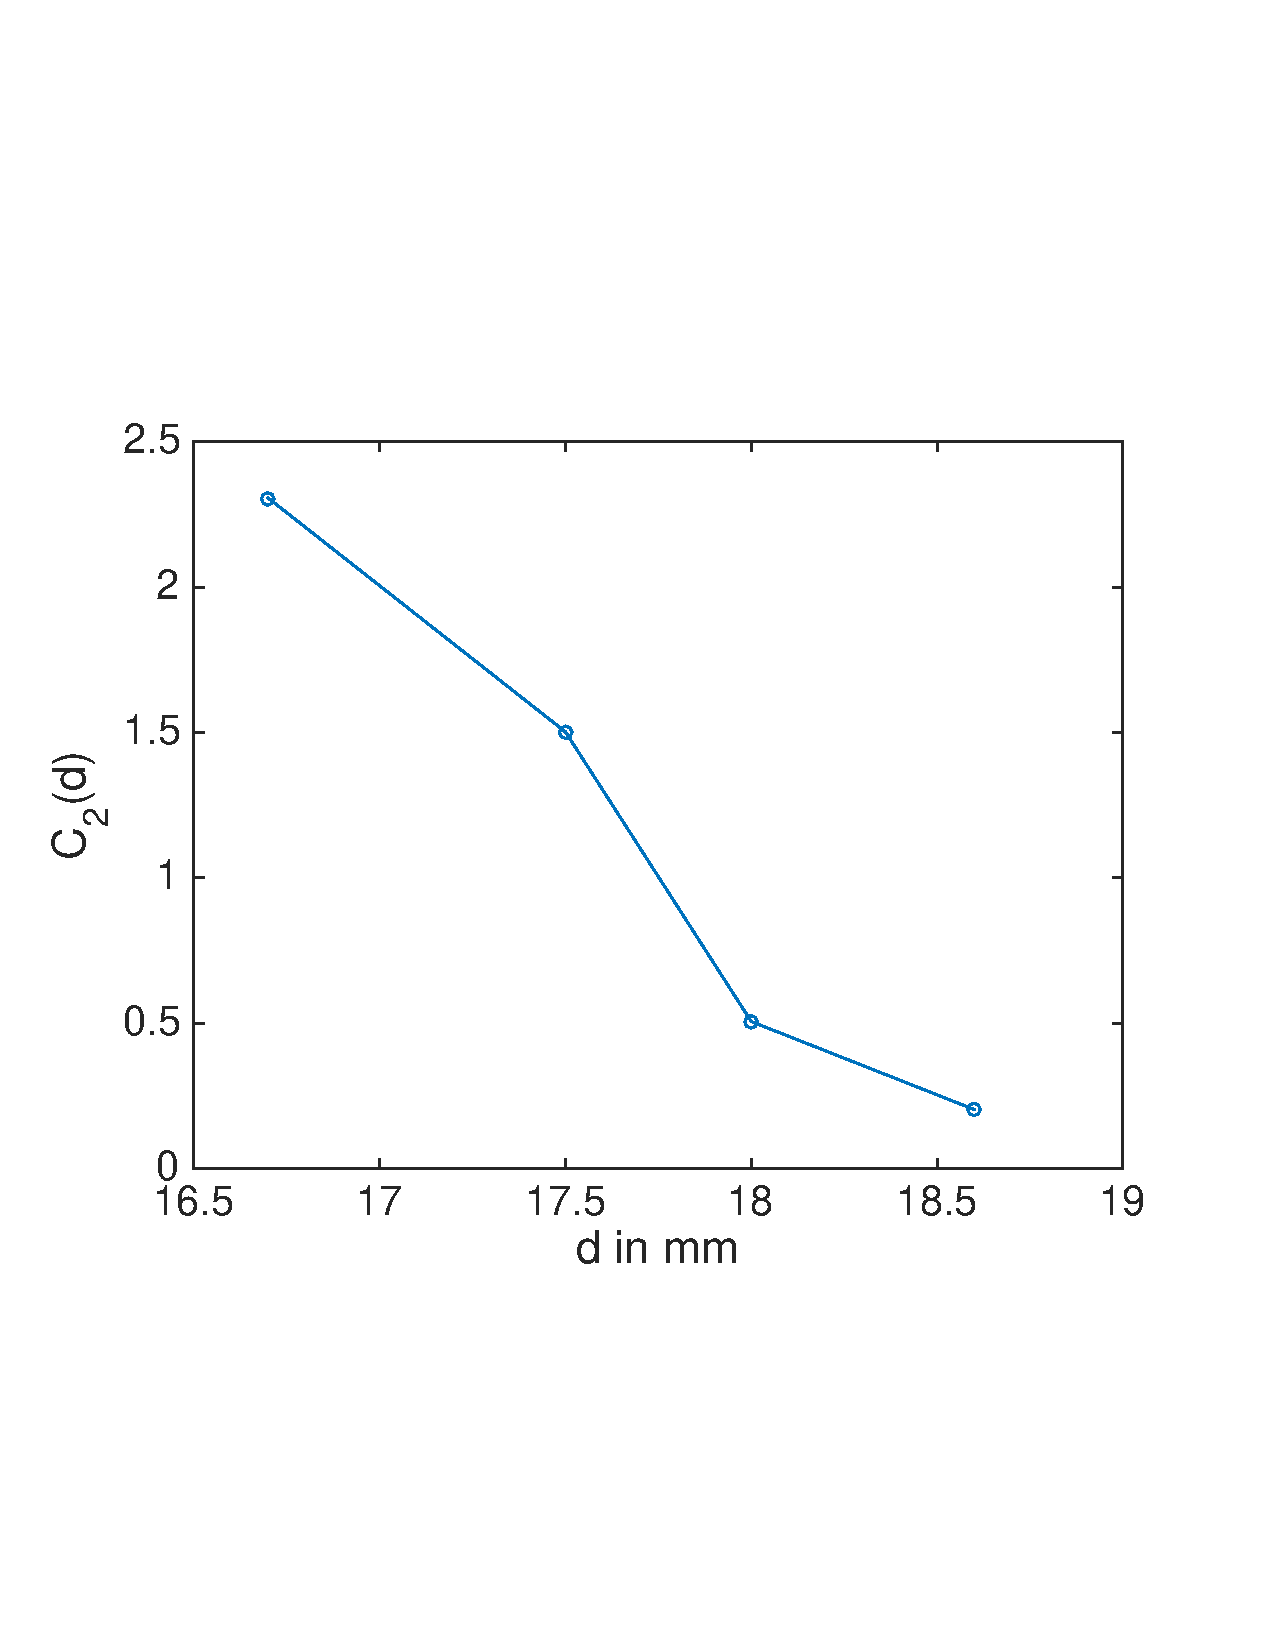
\includegraphics[width=2.5in]{variationC_2}
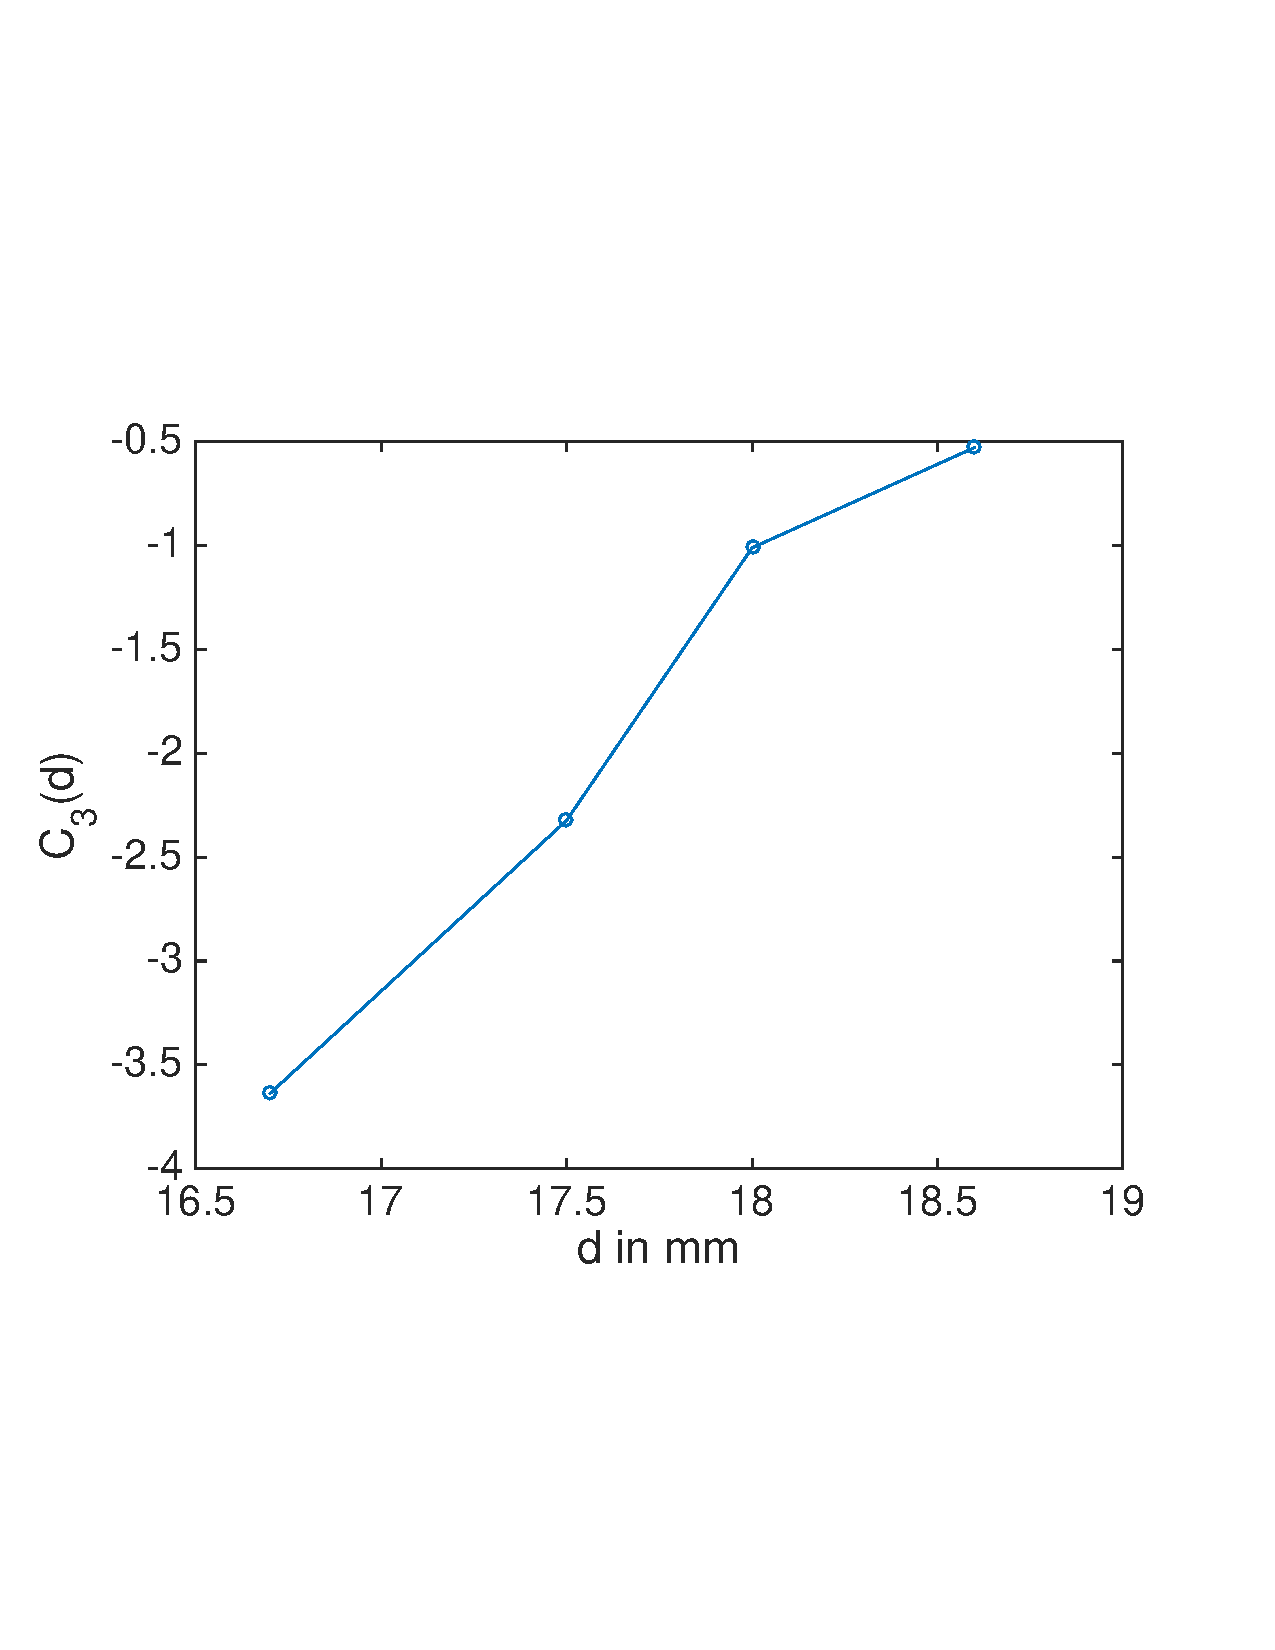
\includegraphics[width=2.5in]{variationC_3}
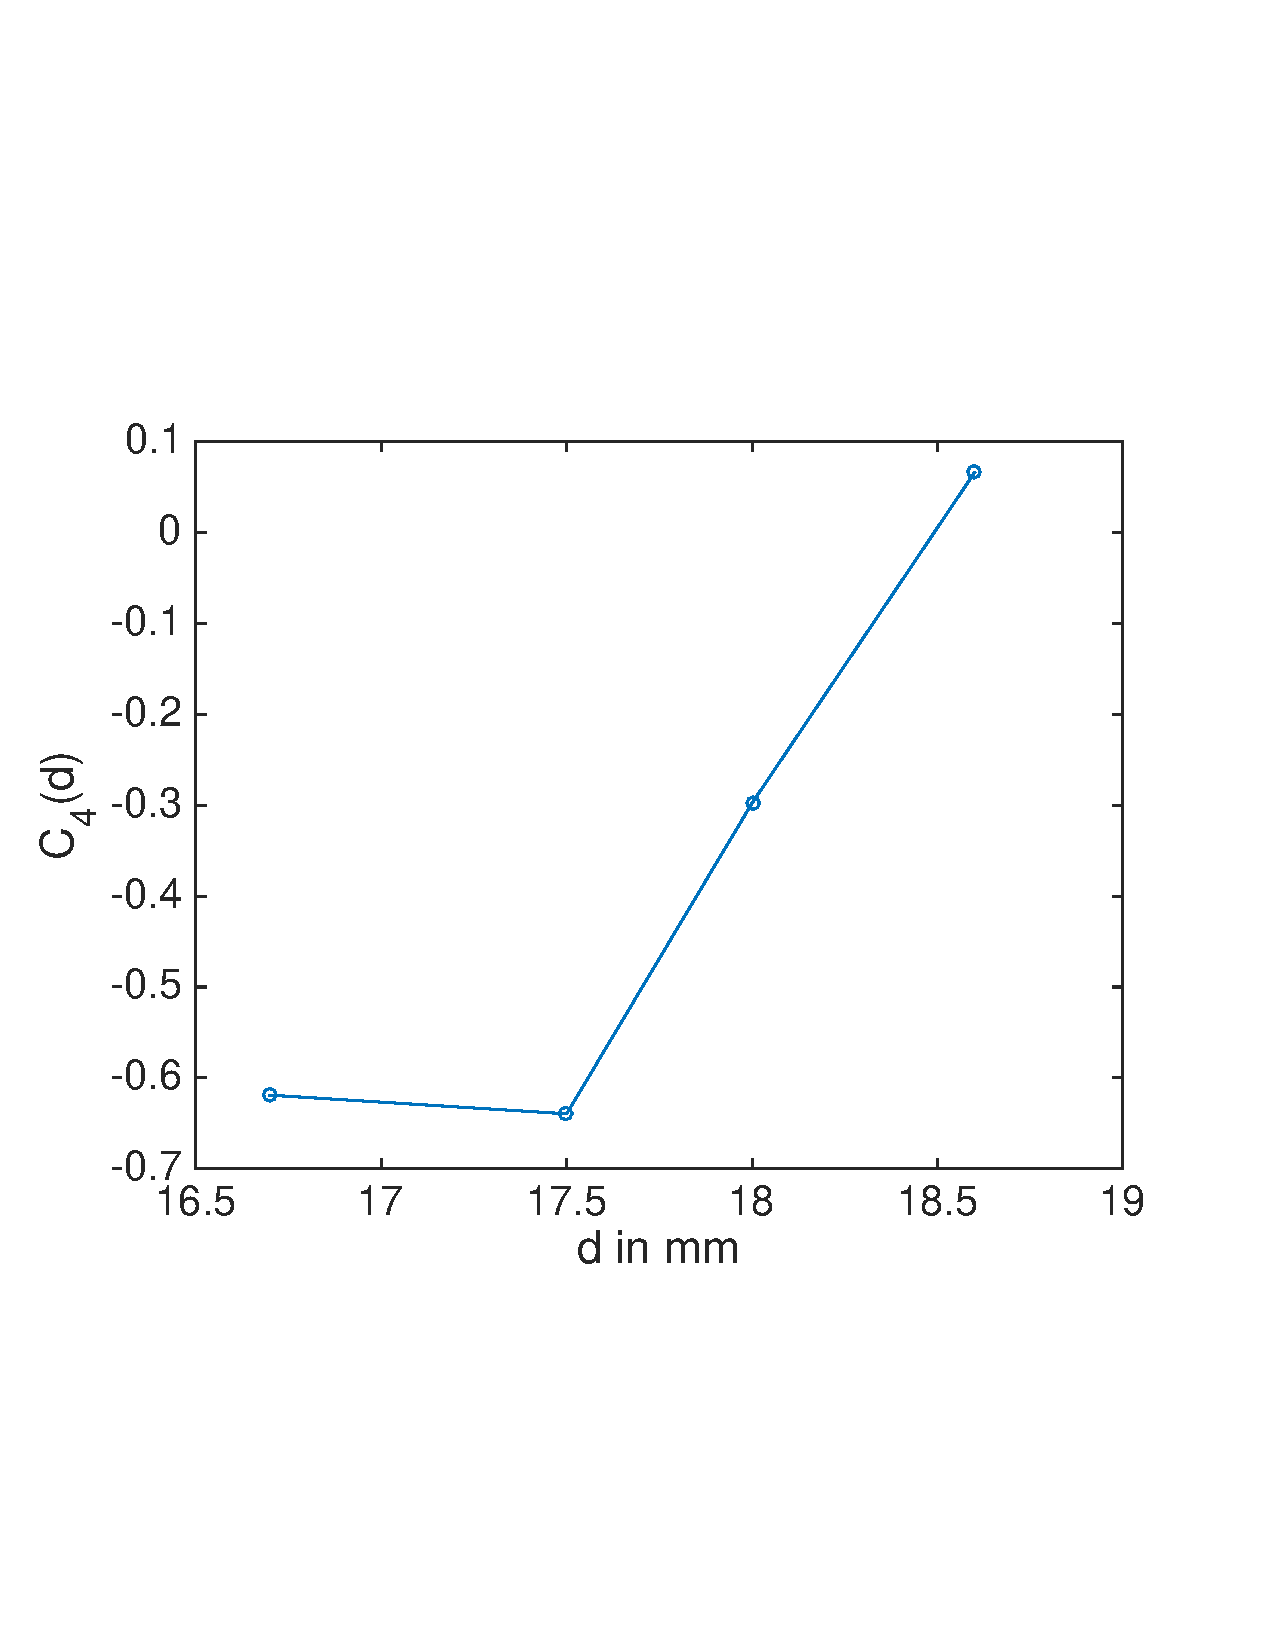
\includegraphics[width=2.5in]{variationC_4}
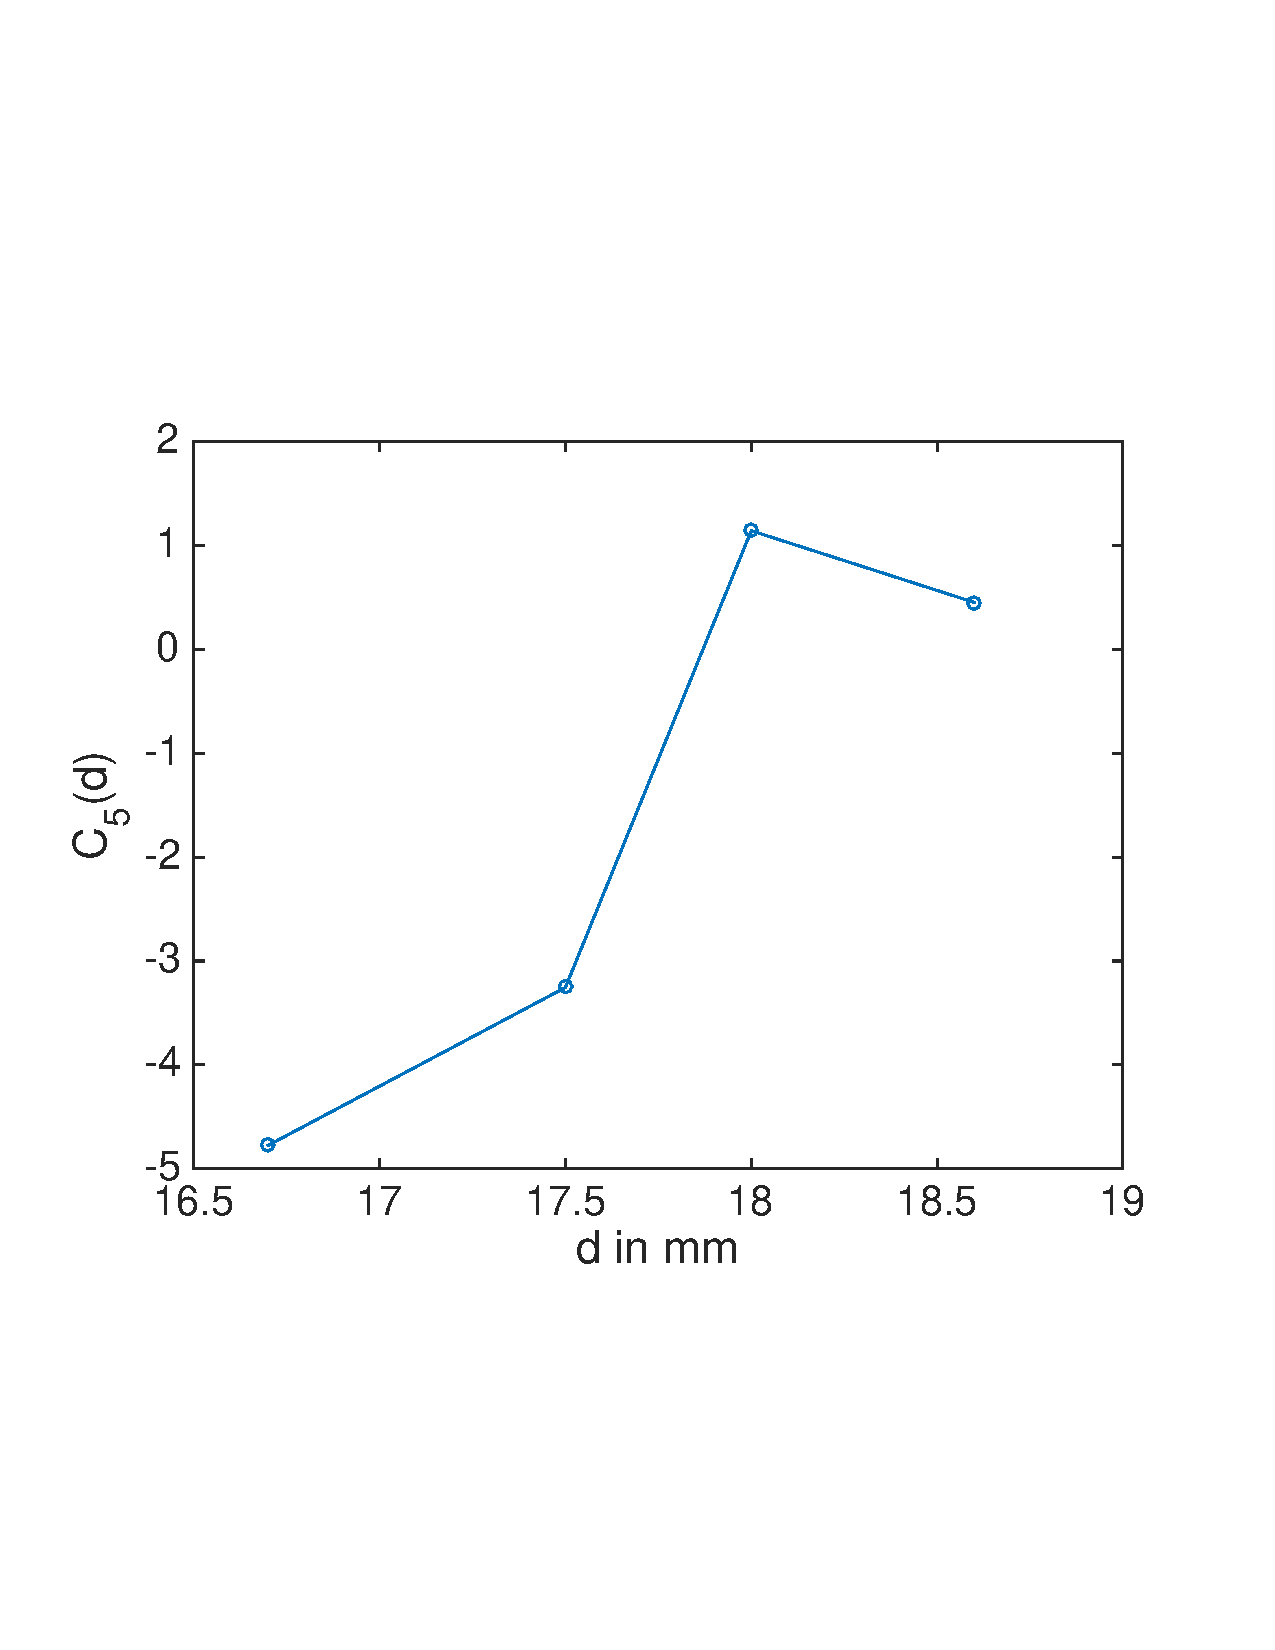
\includegraphics[width=2.37in]{variationC_5}
\caption{Variation of coefficients as a function of $d$.}
\label{fig:coeff1}
\end{figure}
\begin{figure}[h]
\centering
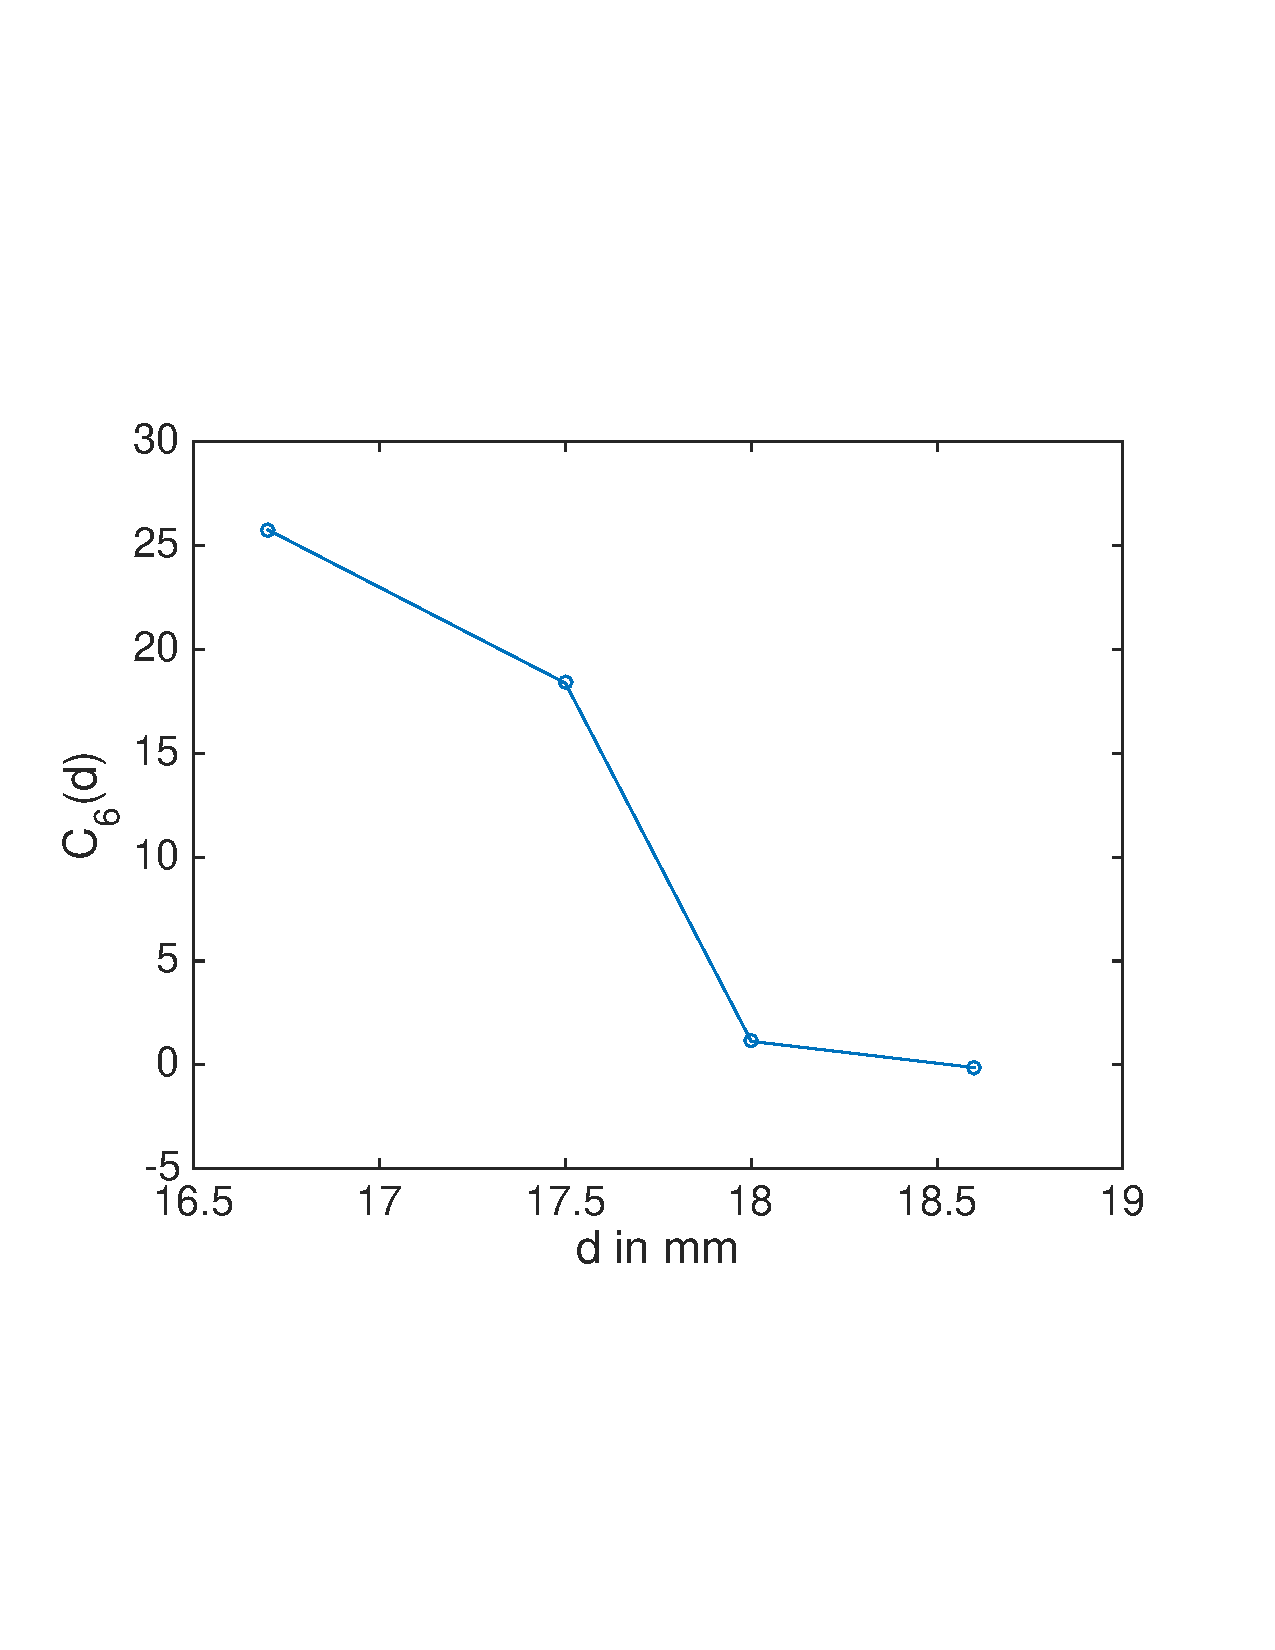
\includegraphics[width=2.5in]{variationC_6}
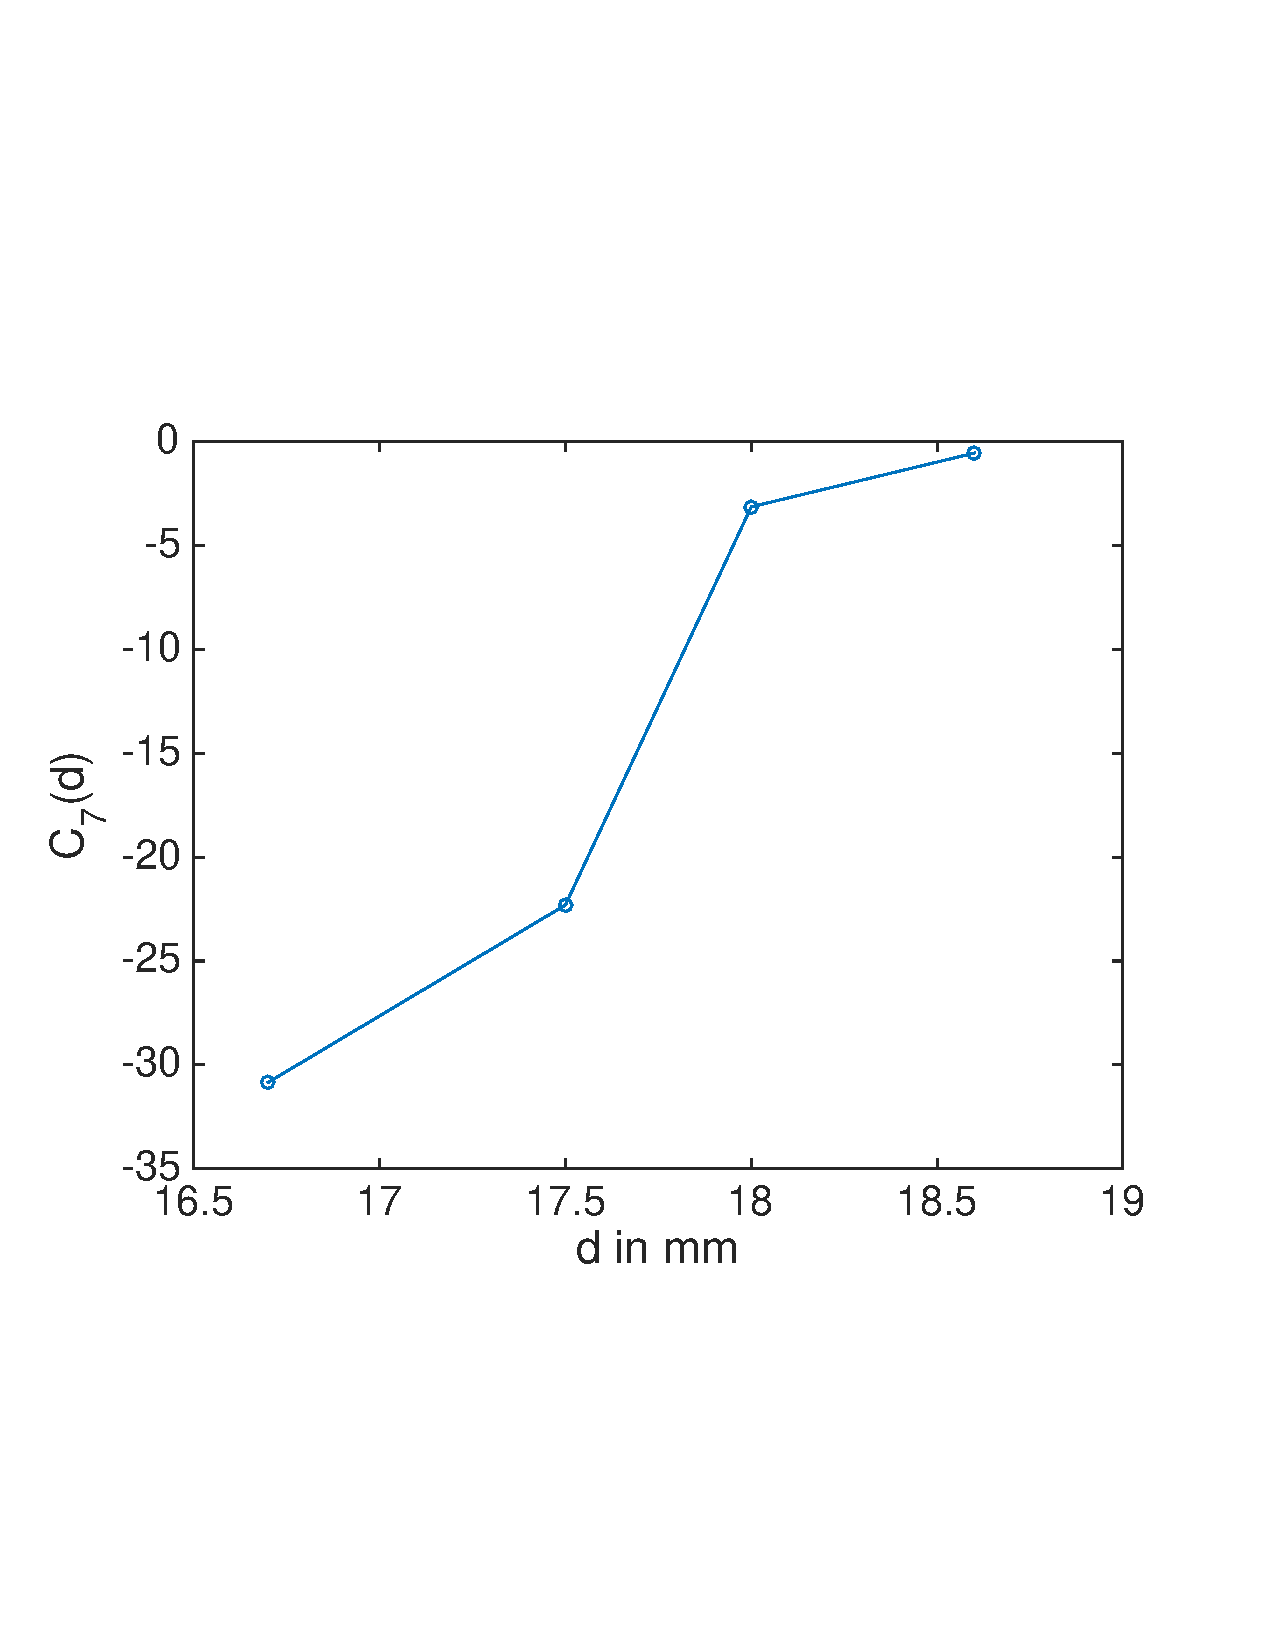
\includegraphics[width=2.5in]{variationC_7}
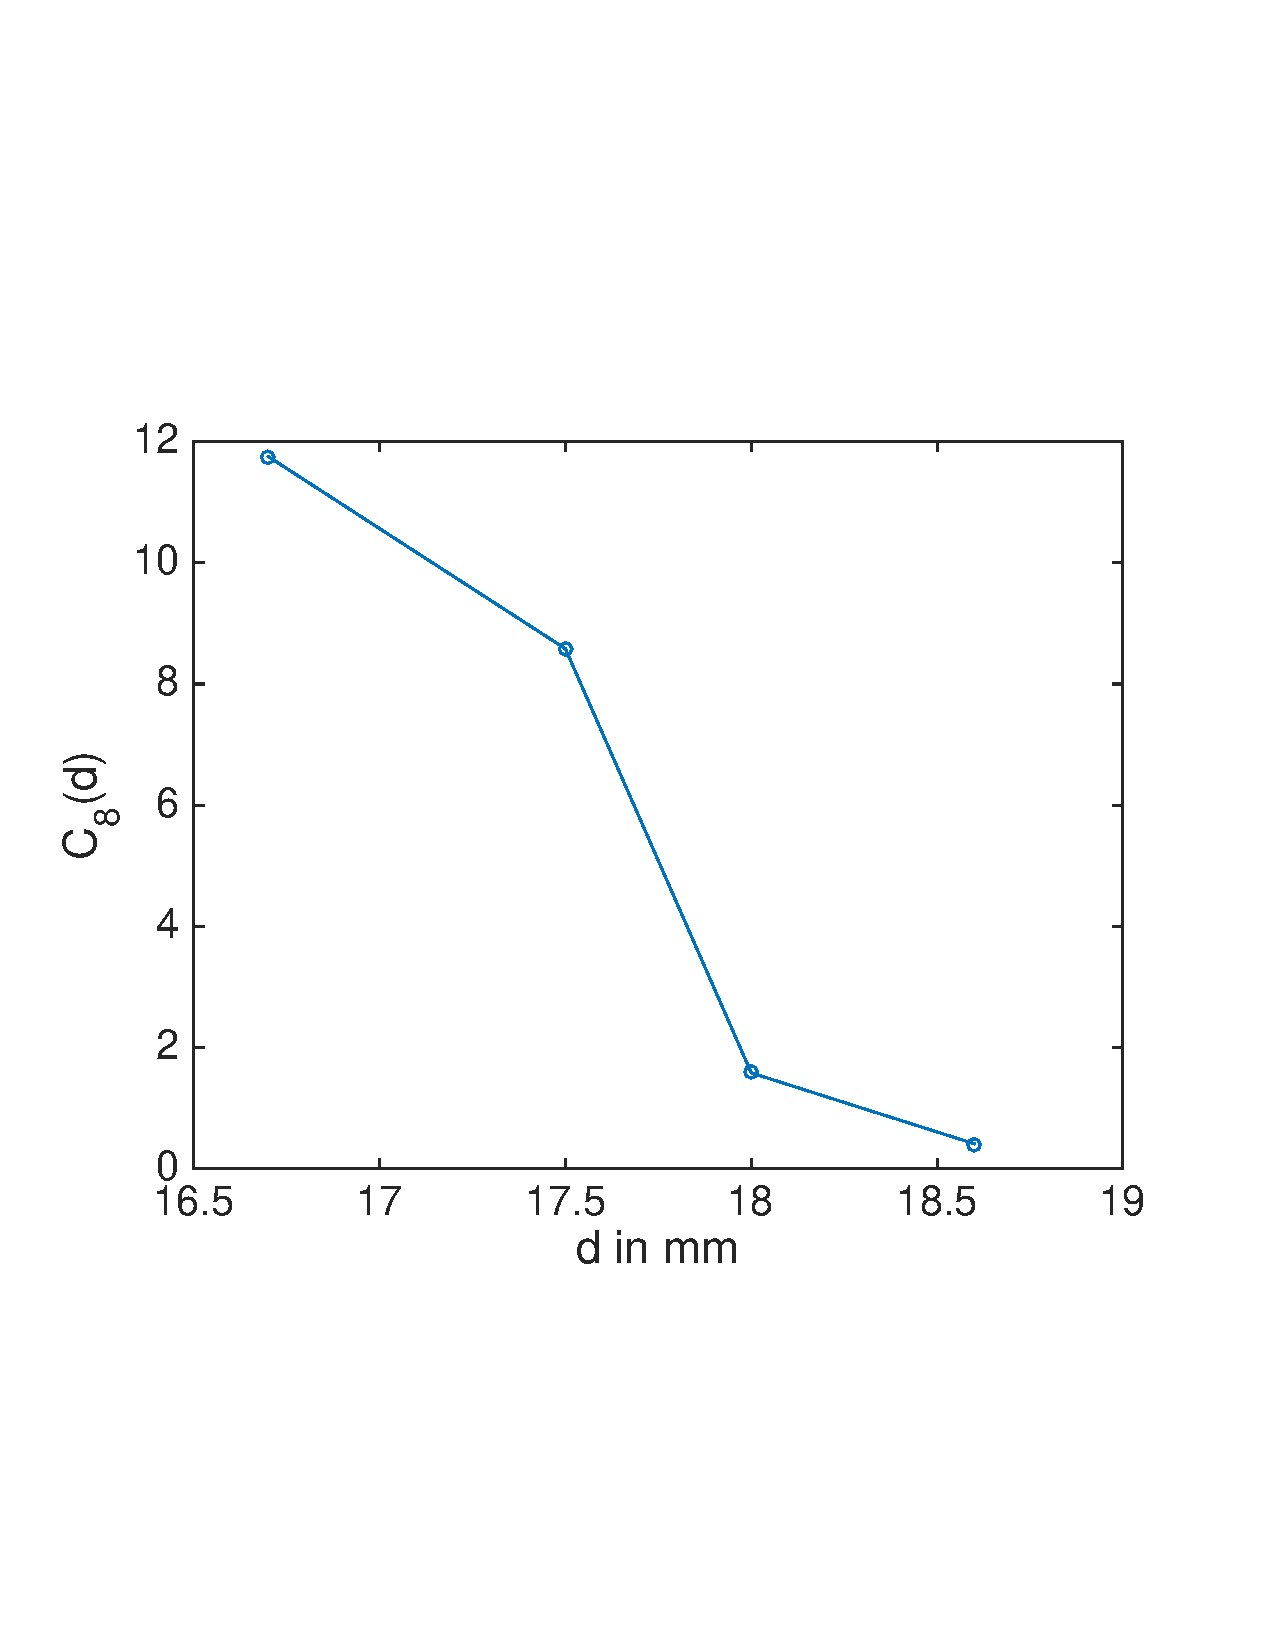
\includegraphics[width=2.5in]{variationC_8}
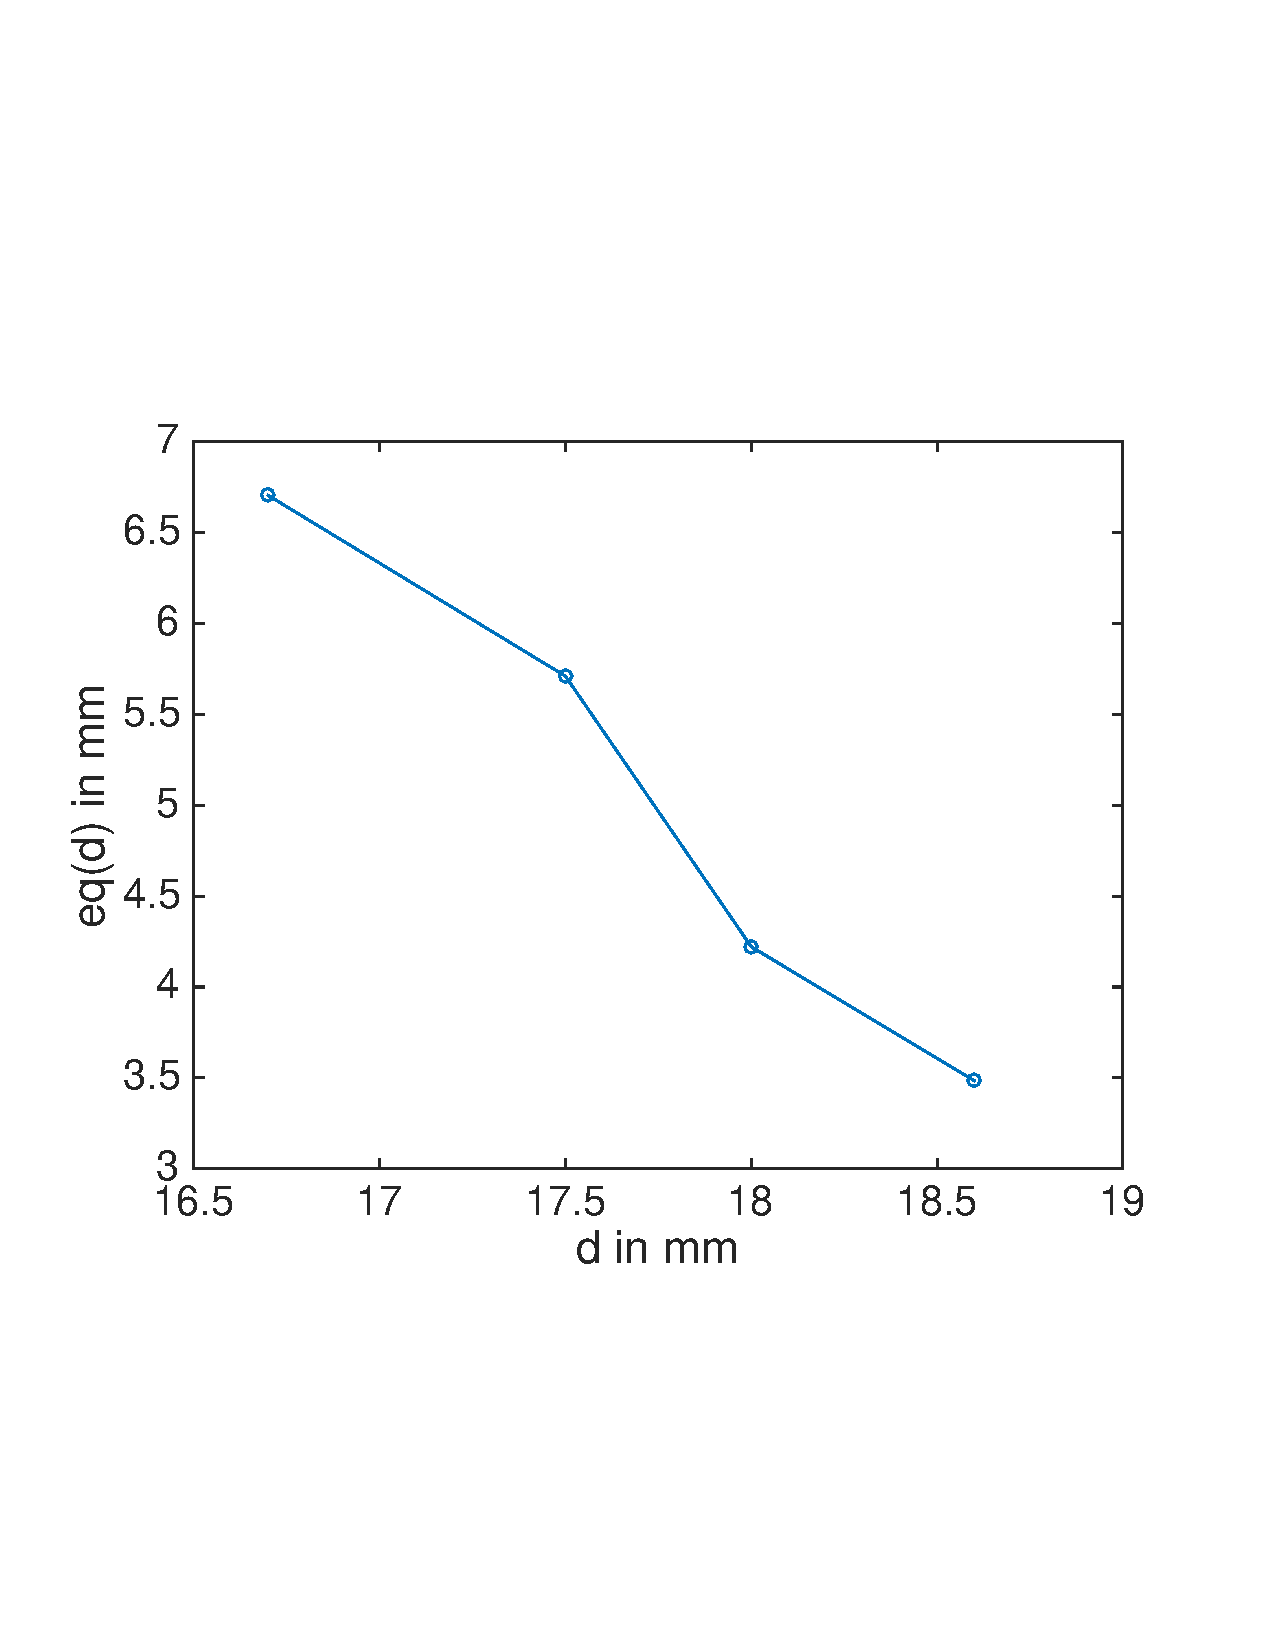
\includegraphics[width=2.5in]{variationEq}
\caption{Coefficients and equilibrium point variation as a function of $d$.}
\label{fig:coeff2}
\end{figure}
It can be seen that there is either an increasing or decreasing general trend in the variation of the coefficients, and the equilibrium point. But, there can be many ways of fitting the parameters e.g. best fit line, quadratic, cubic, etc. In order to figure out the best way to accurately represent the bistable force curve variation with respect to the $d$ parameter, I performed quasi-static simulations of the beam bending problem for various values of $d$. The quasi-static simulations provide numerical force-displacement curves for the bistable beam bending problem as a function of $d$. The results of the same are shown in the following section.

\section{Beam bending quasi-static simulations}
\begin{figure}[h]
\centering
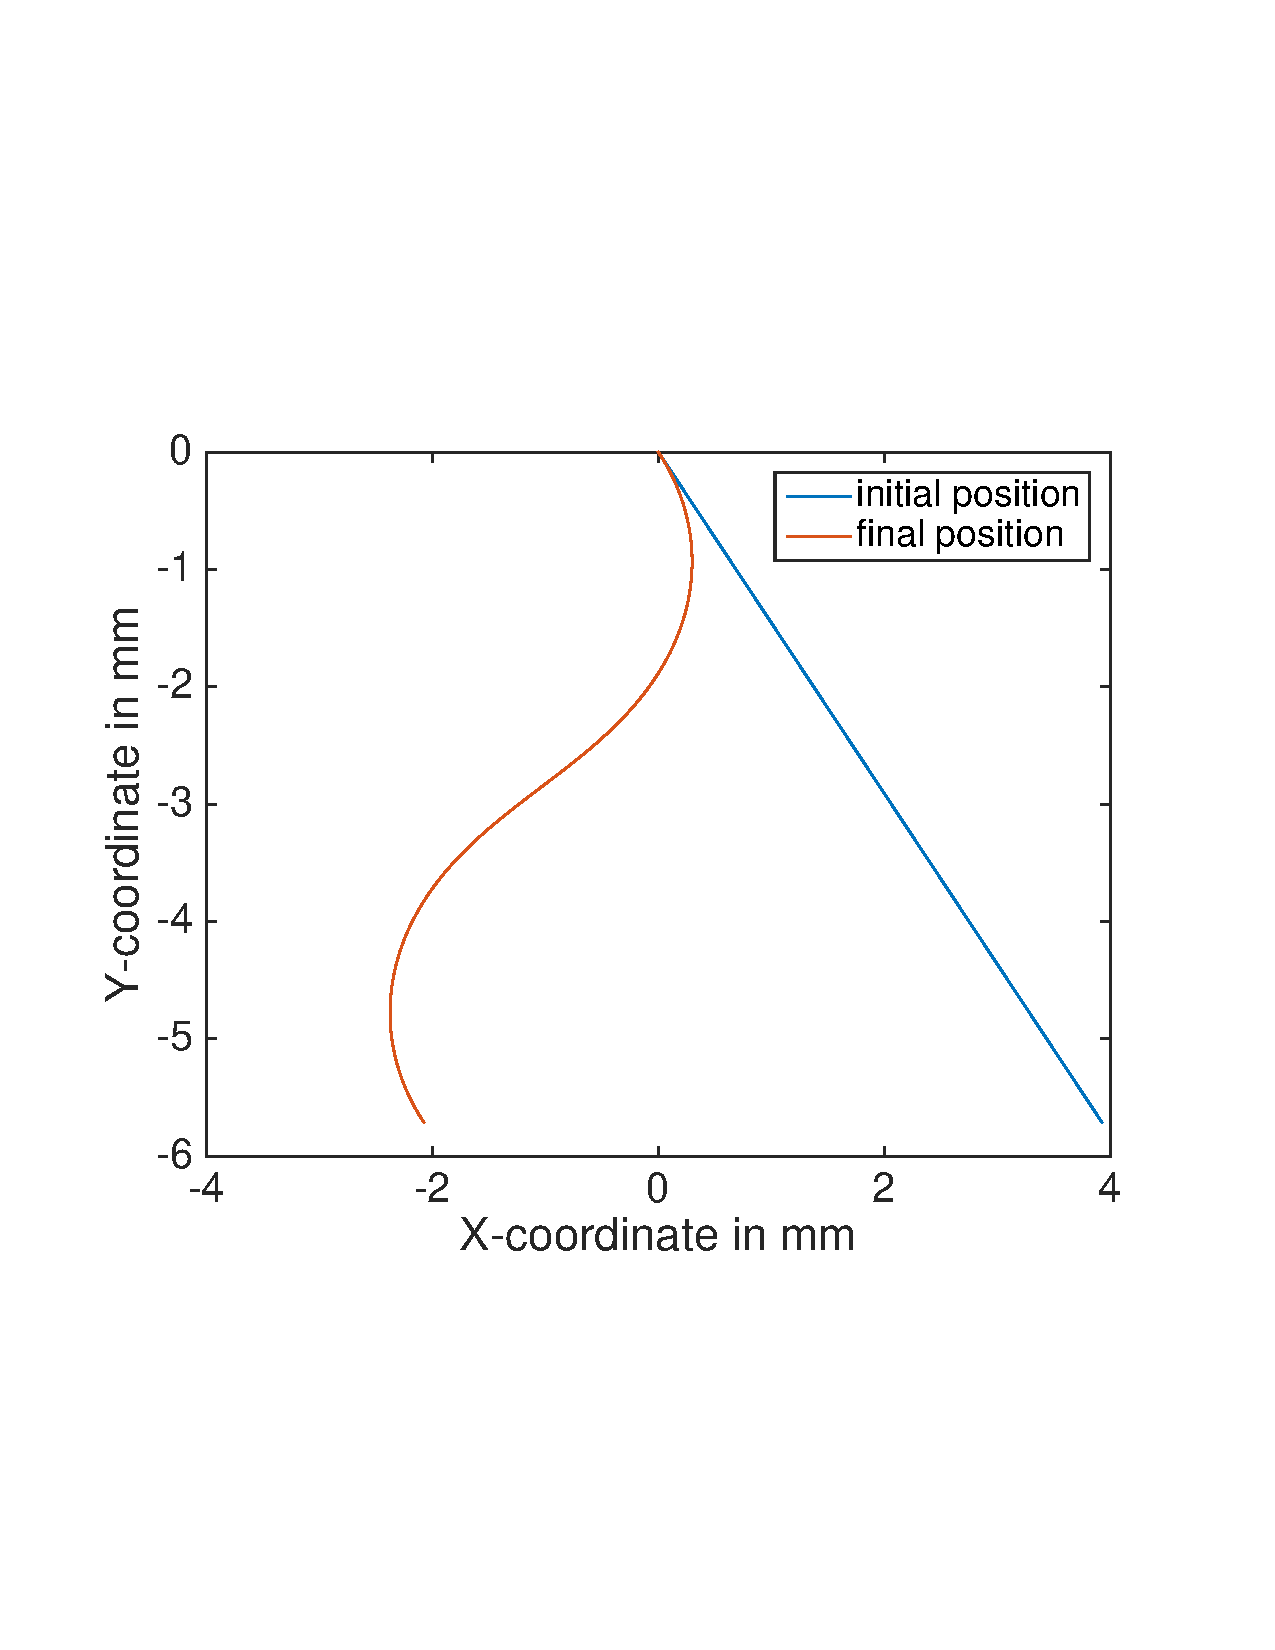
\includegraphics[width=2.5in]{beamBending}
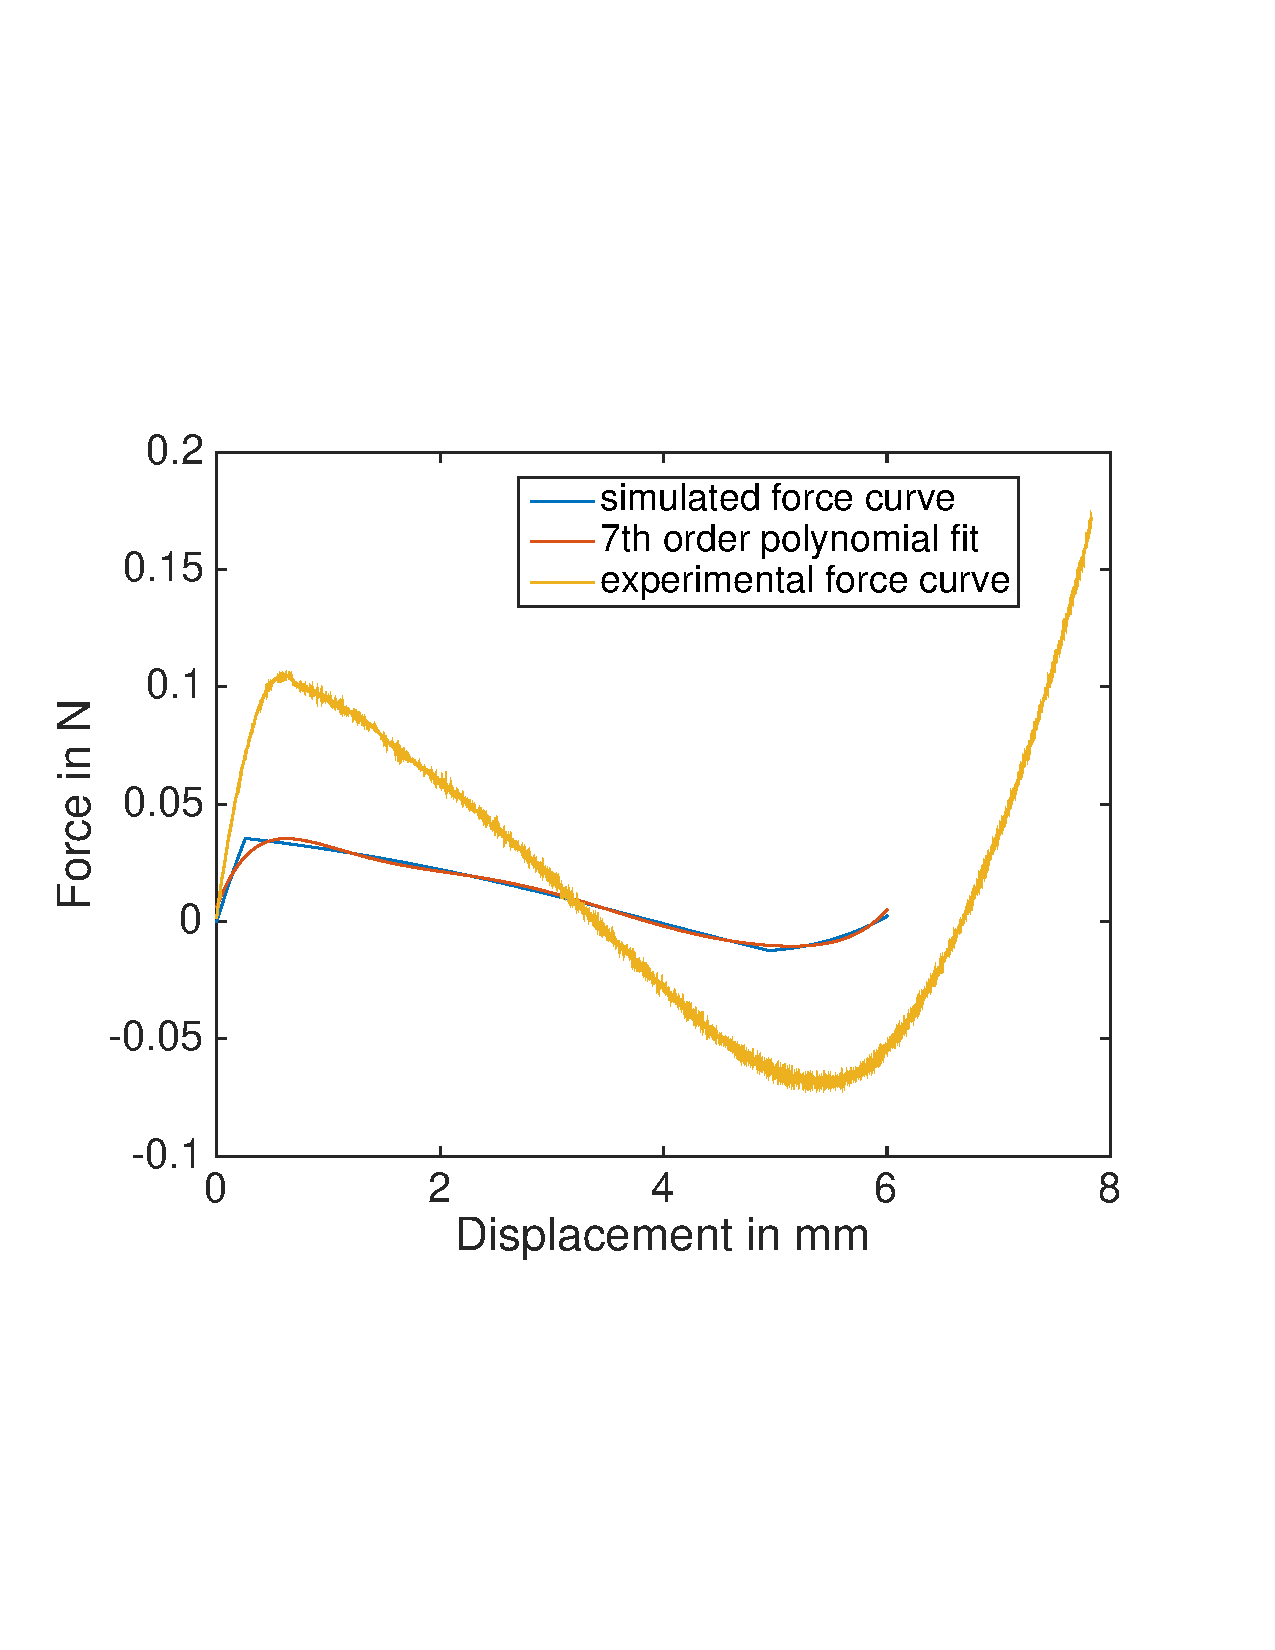
\includegraphics[width=2.5in]{forceDisplacementSimulated}
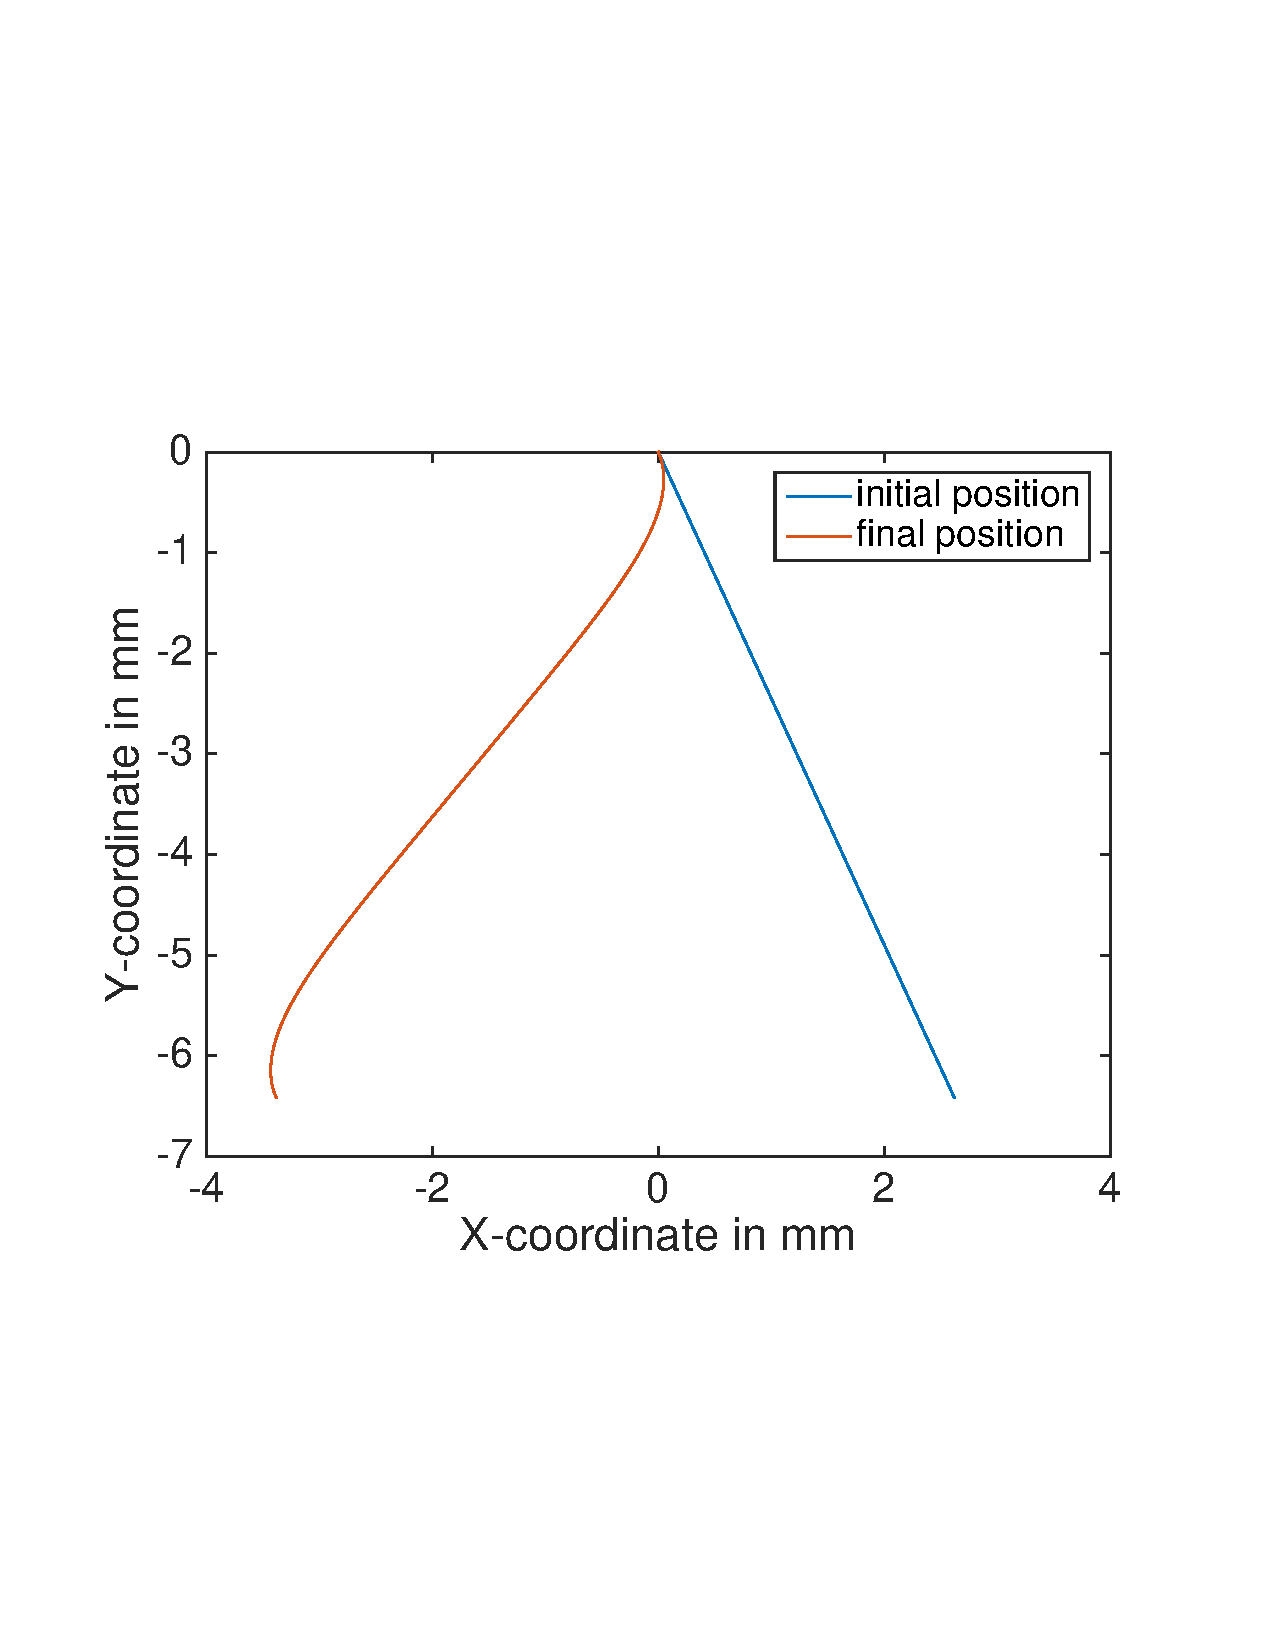
\includegraphics[width=2.5in]{beamBending2}
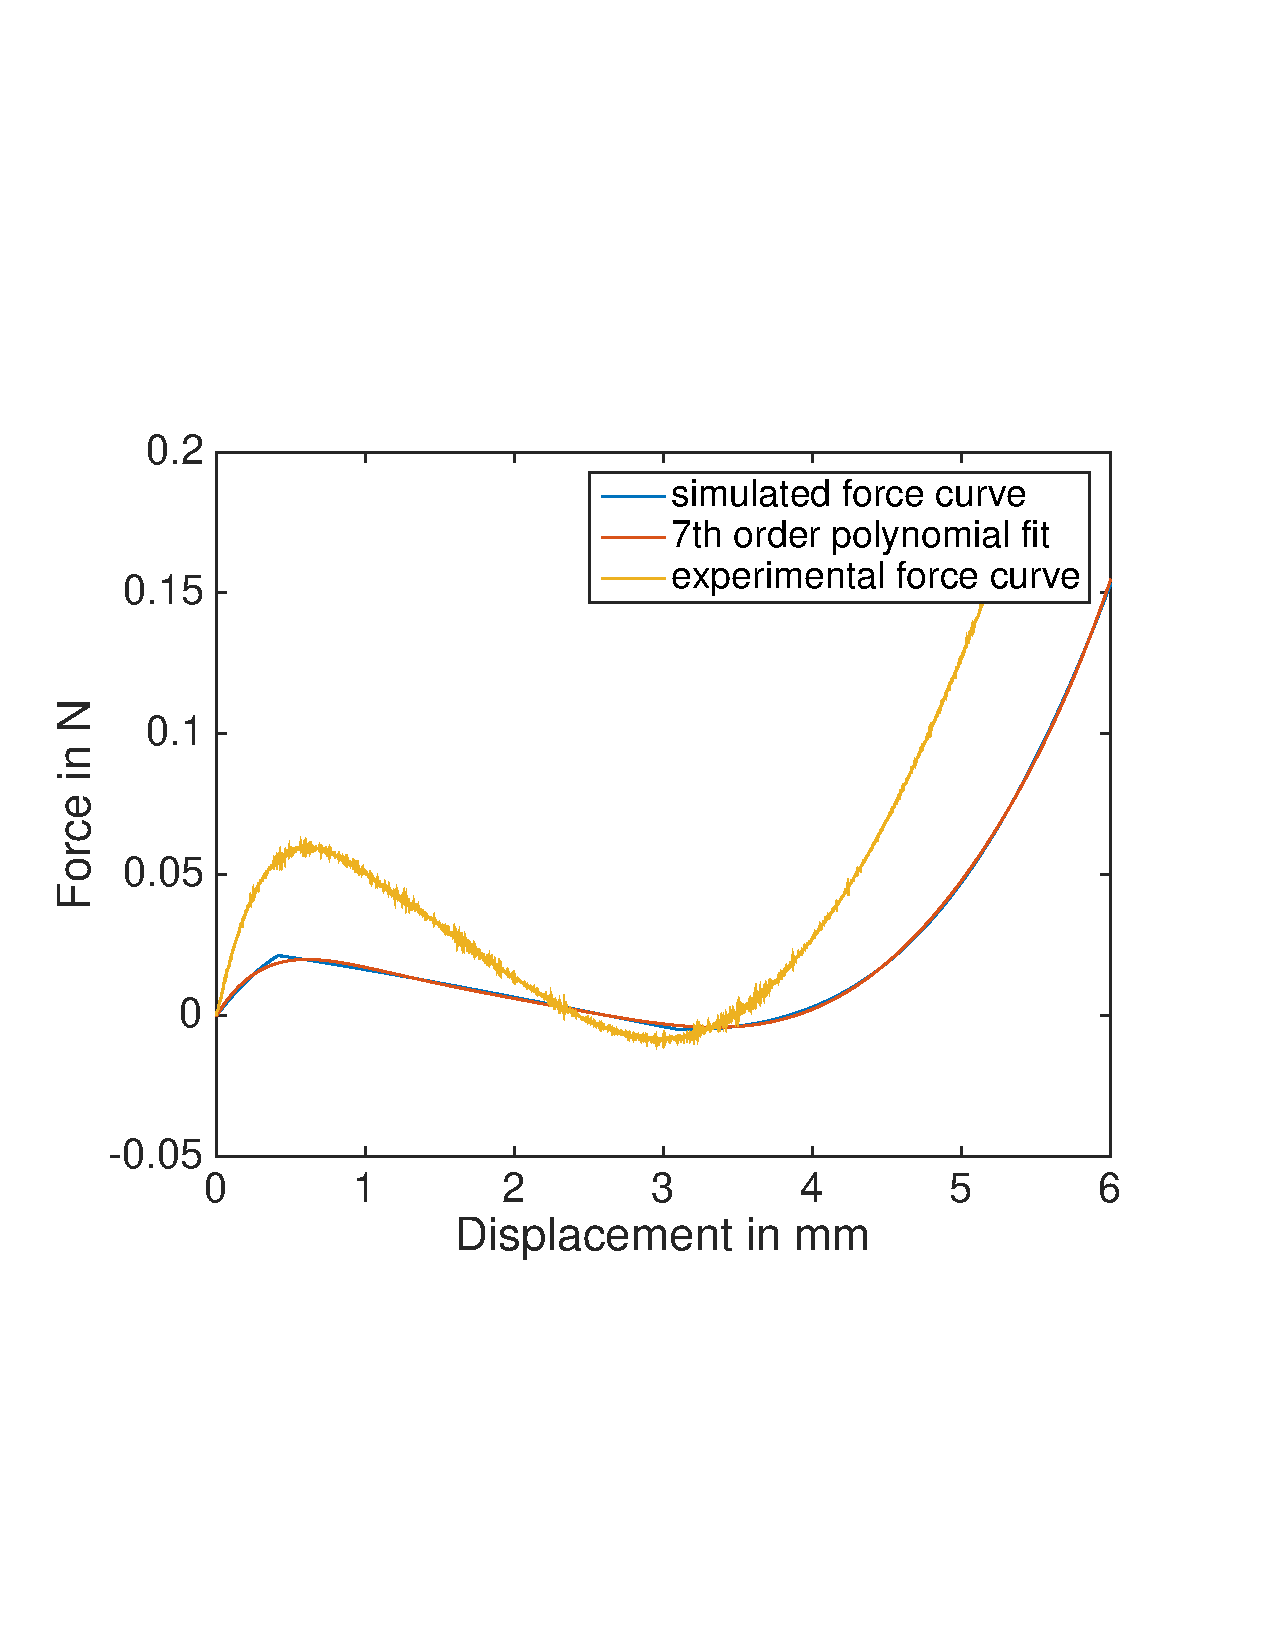
\includegraphics[width=2.5in]{forceDisplacementSimulated2}
\caption{Beam bending quasi-static simulation for $d=18.6$ mm and $d=16.7$ mm.}
\label{fig:simulationQuasiStatic}
\end{figure}
The simulations were performed for one half of the bistable beams. The lowermost node was pushed horizontally and the nodal force was recorded as a function of the displacement. The nodal force was doubled to get the force-displacement curve of the total bistable element. The beam comprised of corotational beam elements that are capable of supporting axial and bending loads. The uppermost node was held fixed without allowing for any rotations. The angle and vertical displacement of the lowermost node was also held fixed. An example quasi-static simulation is shown in Fig.~\ref{fig:simulationQuasiStatic}. The numerically measured force and equilibrium displacement appears to be much smaller than what is expected.

\section{ABAQUS simulations}
Simulations were performed using the ABAQUS software with a Neo-Hookean model with initial Young's modulus ($E_0$) = 0.6 MPa and initial bulk modulus ($\kappa_0$) = 2500$\mu_0$ = 2500$E_0/3$. A sample simulation result of the deformation is shown in Fig.~\ref{fig:simulationAbaqus}.
\begin{figure}[h]
\centering
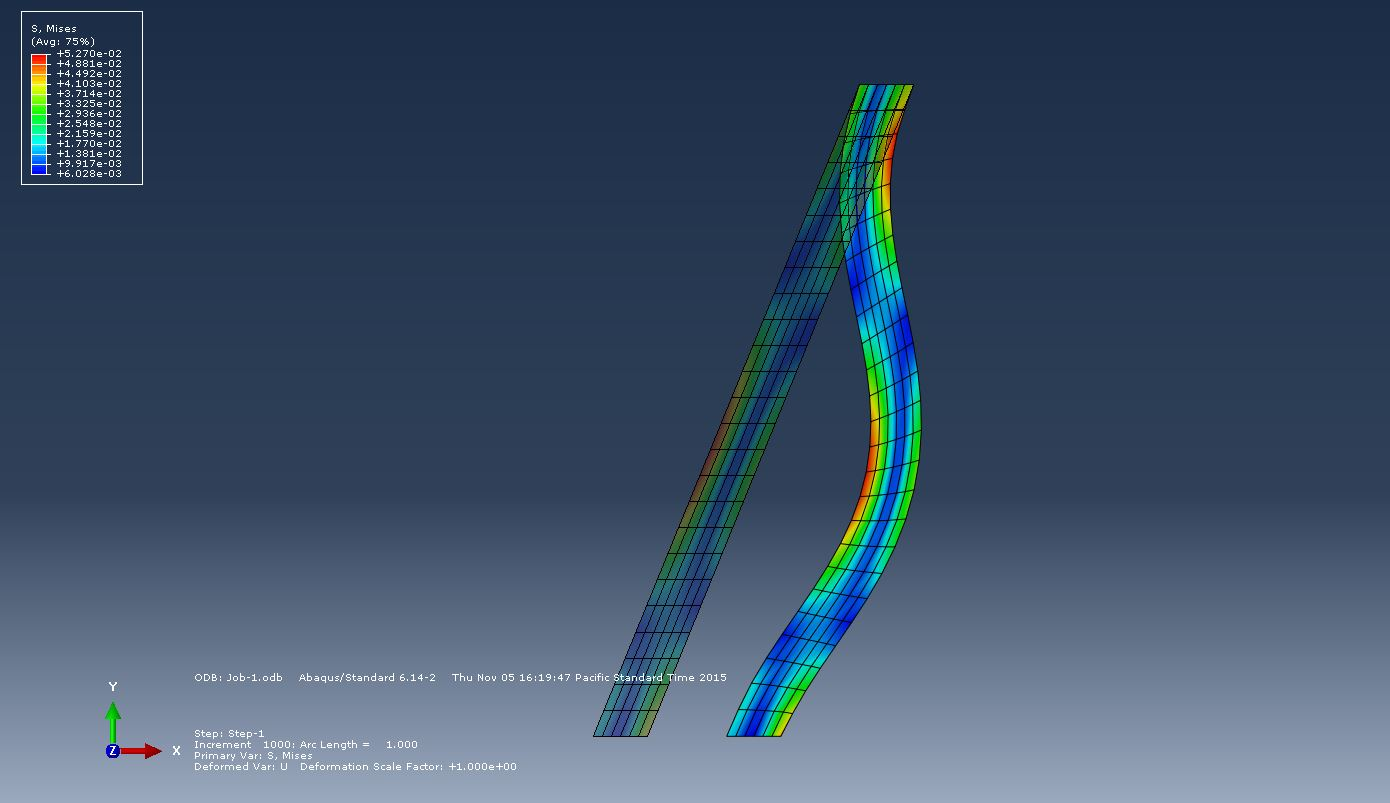
\includegraphics[width=5.5in]{abaqus}
\caption{ABAQUS simulation for $d$ = 16.7 mm}
\label{fig:simulationAbaqus}
\end{figure}

The maximum snapping force was measured using the ABAQUS simulations for all experimental values of $d$. A comparison of the forces measured experimentally, using corotational beams and using ABAQUS are shown in Table 1. It can be seen that the forces are much closer to the corotational beam value than the experimental value.
\begin{table}[h]
\centering
    \begin{tabular}{| c | c | c | c | c |}
    \hline
    $\theta$ in degrees & $d$ in mm & experimental force value & Corotational beam force value & ABAQUS force value \\ \hline
    22.2 & 18.6 & 0.0607 N & 0.0211 N & 0.0174 N \\ \hline
    26.3 & 18 & 0.0692 N & 0.0264 N & 0.0276 N \\ \hline
    32.3 & 17.5 & 0.0921 N & 0.0331 N & 0.0332 N \\ \hline
    34.5 & 16.7 & 0.1049 N & 0.0353 N & 0.0342 N \\
    \hline
    \end{tabular}
    \caption{Table comparing maximum snapping force values between experimental and numerical results.}
\end{table}

\section{Simulations using initial shear modulus $\mu_0 = 0.6$ MPa}
The simulations using an initial shear modulus of $0.6$ MPa are shown in Fig.~\ref{fig:simulationNewWithShearModulus}. The results seem to match very well with the higher value of the shear modulus. 
\begin{figure}[h]
\centering
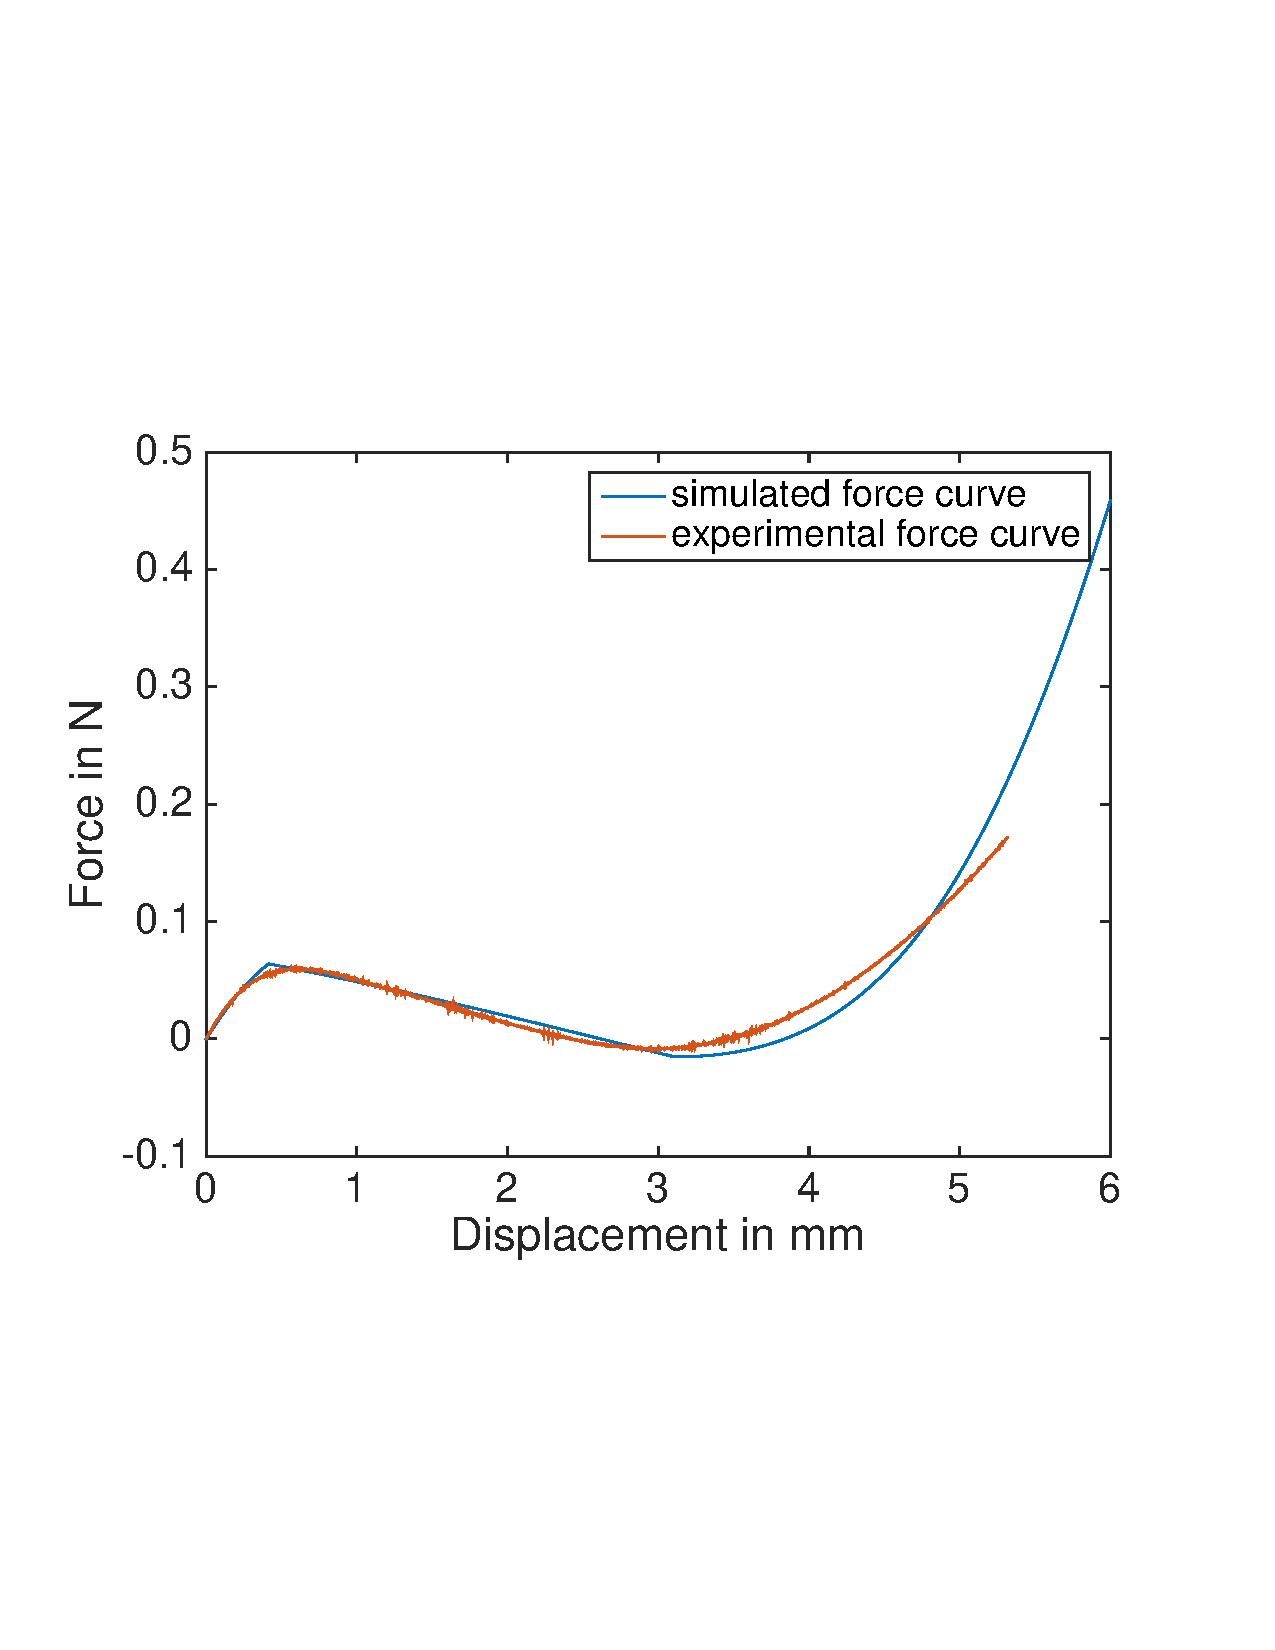
\includegraphics[width=2.5in]{22p2ShearModulusp2}
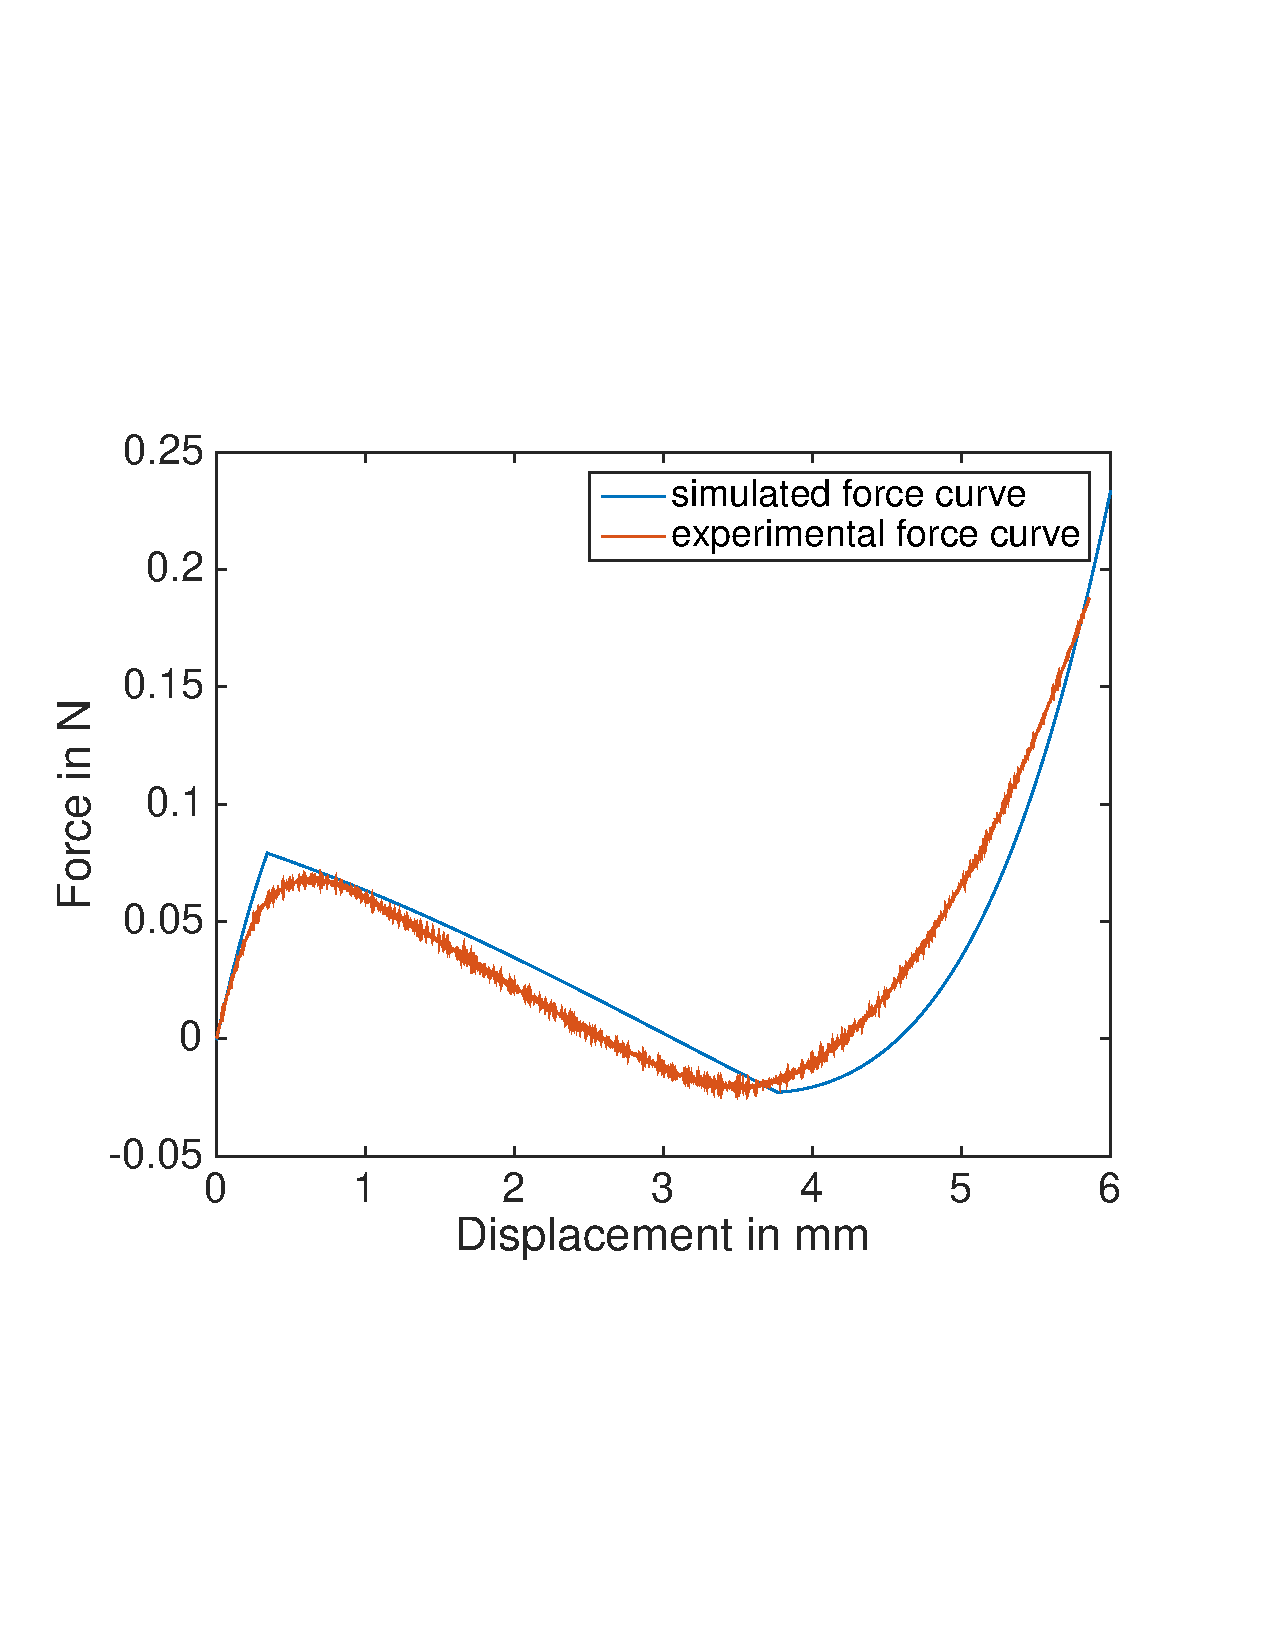
\includegraphics[width=2.5in]{26p2ShearModulusp2}
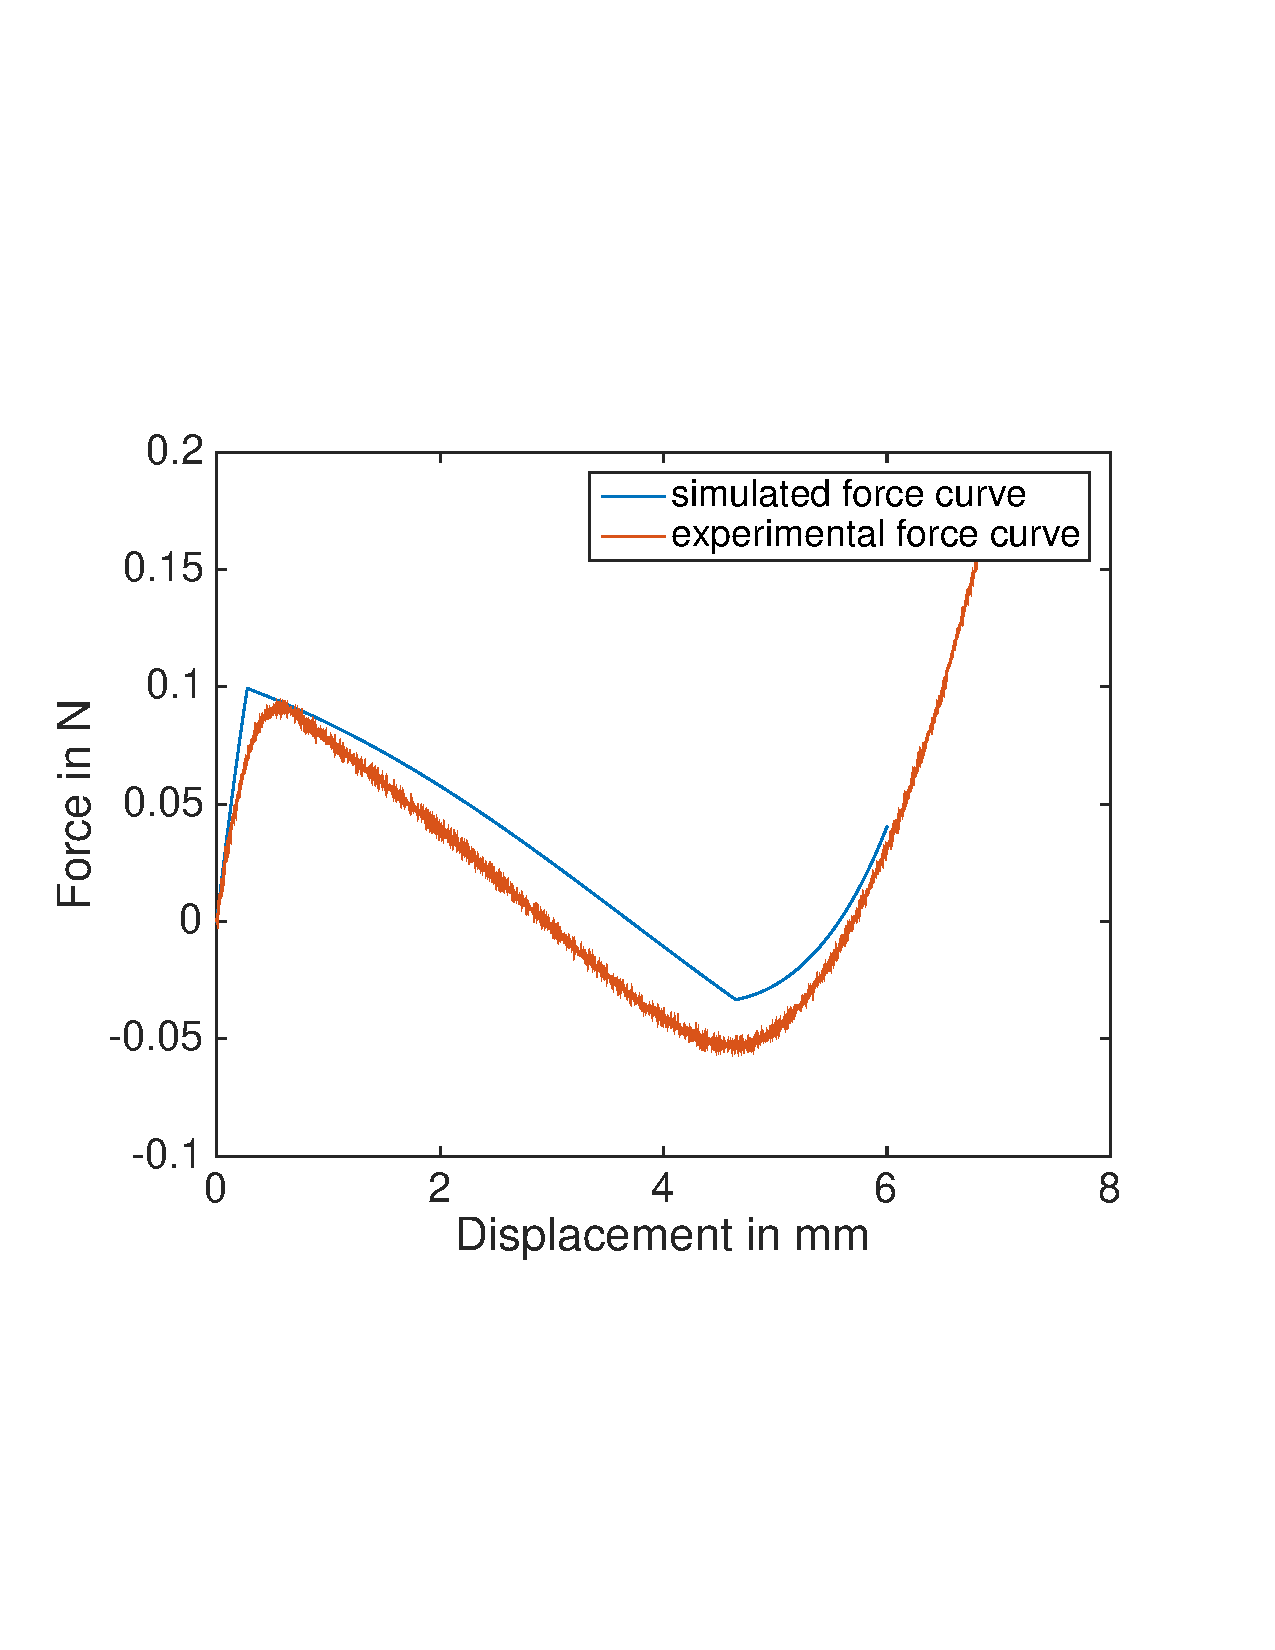
\includegraphics[width=2.5in]{32p3ShearModulusp2}
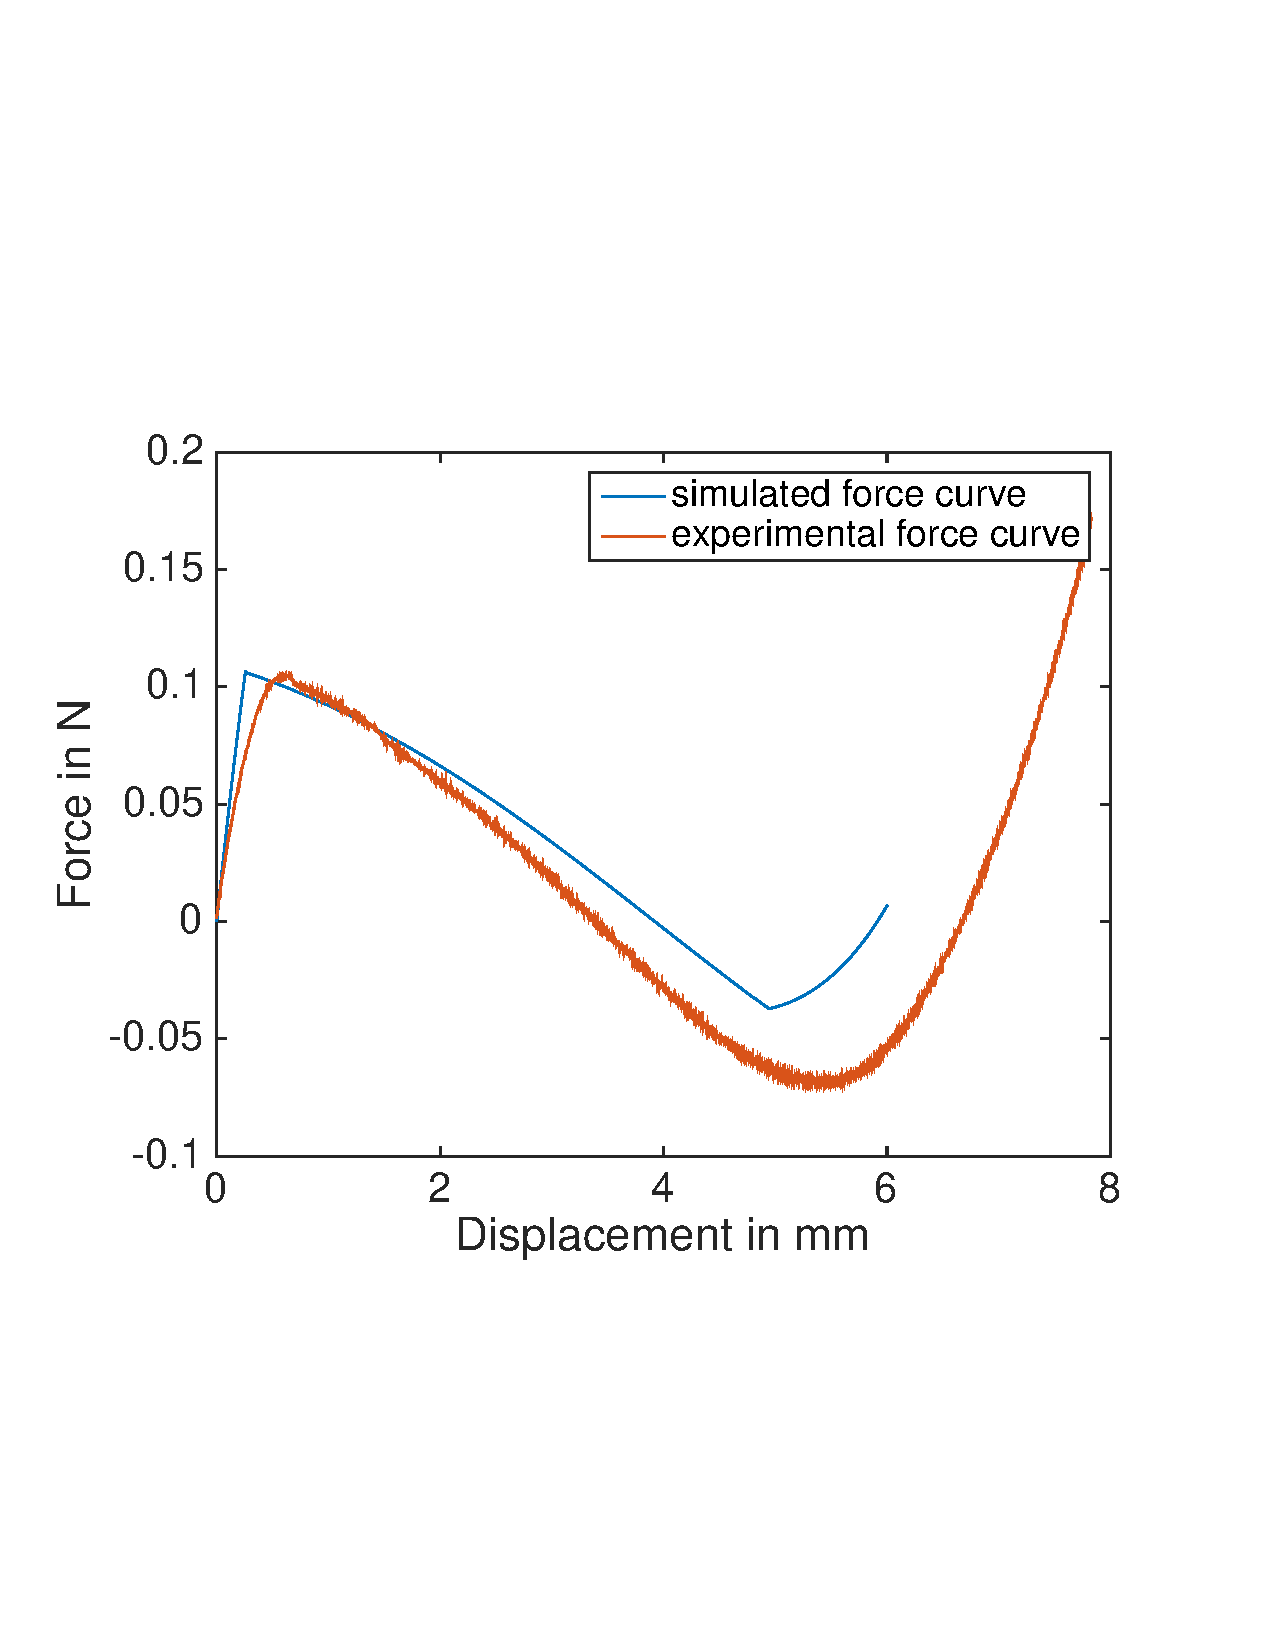
\includegraphics[width=2.5in]{34p5ShearModulusp2}
\caption{Beam bending simulations for all experimental values: (a) 18.6 mm, (b) 18 mm, (c) 17.5 mm, (d) 16.7 mm}
\label{fig:simulationNewWithShearModulus}
\end{figure}
\end{document}